%
% METU Institute of Natural and Applied Sciences Thesis example 
%
% Edited and Commented by Utku Erdoğdu 2013
% Modified for IAM - Institute of Applied Mathematics
% Graduate School of Applied Mathematics
% Edited and Commented by Omur Ugur 2017-2018
%
% Please read the explanations so that you can customize the document		
%
% Files needed by this document:
% metu.cls 
% metu11.def (if you will use 11pt fonts) 
% metu12.def (if you will use 12pt fonts)
% metu10.def (if you will use 10pt fonts)
%
% Possible Options Here:
%
% oneandhalf, double, single : Line spacing used in the thesis. 
% Default and institute preference is
% single.
%
% 10pt, 11pt, 12pt : Font size Default is 10pt, which is institue choice. 
% 
% pntr, pntc, pnbt : Page number position. 
% Options are top center, top right or bottom. 
% Default and institute preference is page numbers at bottom. 
% When page numbers are at the top bottom margins are skewed.
% 
% chaproman, chaparabic: Chapter numbering format. 
% Options are roman numbers and arabic numbers.
% Default is roman, institute prefers arabic
%
% oneside, twoside : Printing style. Default is twoside. 
% In this style chapters and (almost all) preliminary pages begin from 
% odd numbered pages.
%
% tr, eng : Document language. This is useful if you want to translate 
% your thesis into Turkish. 
% Then you give the option tr and use \ifturkish. . .\else. . .\fi  
% whenever you want 
% to do something only for Turkish or only for English. Default is eng. 
% IMPORTANT!! : For official institute documents you should not use this option. 
% The Turkish format is only supplied for custom translations.
%
% ceng,aee,arme.. : You can use the abbreviated form of your department here 
% and there is no further need to define the department name below. 
% If your department name is not among the below list of defined
% departments, you should use \department and \turkishdepartment macros 
% to define the name of your department.
%
% Defined Departments and Abbreviations:
% (may not work after modification for IAM)
% --------------------------------------
% Computer Engineering : ceng
% Aerospace Engineering : aee
% Archaeometry : arme
% Architecture : arch
% Biochemistry : bch
% Biology : biol
% Biomedical Engineering : bme
% Biotechnology : btec
% Building Science : bs
% Cement Engineering : ceme
% Chemical Engineering : che
% Chemistry : chem
% City and Regional Planning : crp
% City Planning : cp
% Civil Engineering : ce
% Computational Design and Fabrication Technologies in Architecture : arcd
% Computer Education and Instructional Technology : cte
% Design Research for Interaction : iddi
% Earthquake Studies : eqs
% Earth System Science : ess
% Electrical and Electronics Engineering : ee
% Engineering Management : em
% Engineering Sciences : es
% Environmental Engineering : enve
% Food Engineering : fde
% Geodetics - Geographical Information Technologies : ggit
% Geological Engineering : geoe
% Hydrosystems Engineering : he
% Industrial Design : id
% Industrial Engineering : ie
% Mathematics : math
% Mechanical Engineering : mech
% Metallurgical and Materials Engineering : mete
% Micro and Nanotechnology : mnt
% Mining Engineering : mine
% Operational Research : or
% Petroleum and Natural Gas Engineering : pete
% Physics : phys
% Polymer Science and Technology : pst
% Regional Planning : rp
% Restoration : rest
% Secondary Science and Mathematics Education : ssme
% Software Engineering : se
% Statistics : stat
% Structural Mechanics : st
% 
% phd, ms : Degree Received. Ph.D. or M.S. Default is M.S.
%
%
% Defined for use of IAM:
% acsc, cryp, fm, sc
%
% End of Options


% Use one of the following \documentclass with options of metu_iam.cls
\documentclass[chaparabic,sc,ms,12pt,oneandhalf]{metu_iam} 
%\documentclass[chaparabic,fm,ms,11pt,oneandhalf]{metu_iam} % preferred by IAM
%\documentclass[chaparabic,acsc,ms,10pt,single]{metu_iam} % preferred by the FBE
%\documentclass[chaparabic,cryp,phd,12pt,double]{metu_iam}

% You can delete next line If your thesis does not have an appendix
\usepackage{appendix}

%
% Personal Information 
% ----------------------------
%
% Please check this part and fill in information about your thesis
%
% Name and Surname
% be careful with the uppercase letters and Turkish characters
% following name should work for both UPPERCASE and LOWERCASE names
\author{\.{I}sa Eren Y\i{}ld\i{}r\i{}m} 
% Thesis Title English and Turkish
\title{Traveltime Tomography Harnessing Physics Informed Neural Networks}
\turkishtitle{Fizik Bilgili Sinir Ağları Kullanan Seyehat S\"{u}resi Tomografisi}
% Department : English and Turkish
%
% Some of the departments are pre-defined, you need not redeclare them. 
% You can use them by just giving an option to \documentclass. 
% See documentation for options above. If you will define your 
% department here do not use ``Department'' or ``Bölümü'' words.
%\department{Computer Engineering}
%\turkishdepartment{Bilgisayar Mühendisliği}
%
% Date : You should indicate the month of your thesis defence in English.
% Default is this month
%
\date{November 2021} % do NOT use comma
%
% Approval Page Details
% --------------------------
% For each command you can give the title as optional parameter enclosed in [ ]
% This also handles the Turkish titles if you're planning 
% to produce Turkish version of the document. 
% If you'll hard code the title, you need 
% to use turkish version of each command after the command itself
% 
% prof : Prof. Dr.
% assocprof : Assoc. Prof. Dr.
% assistprof : Assist. Prof. Dr.
% dr : Dr.
%
% Director of Institute
\director[prof]{A. Sevtap Sel\c{c}uk-Kestel}
% Head of Department
\headofdept[assocprof]{Hamdullah Y\"{u}cel}
%
% Supervisor : English and Turkish
\supervisor[prof]{\"{O}m\"{u}r U\u{g}ur}
\cosupervisor[assistprof]{Umair bin Waheed} % suppress/comment if you don't have cosupervisor
% \turkishsupervisor{  } %if you will hard-code the academic title
%
% Affiliation of Supervisor in English and possibly in Turkish
\departmentofsupervisor{Scientific Computing, METU}
% \turkishcosupervisor{Prof. Dr. Reda Alhajj} %if you will hard-code the academic title
% Affiliation of Co-Supervisor
% You can just delete/comment the next line if you don't have a co-supervisor
\departmentofcosupervisor{Department of Geosciences, KFUPM}
%
% Committee Members
% In general members are sorted according to their academic titles; however
% new modifications indicate
%
% The Chair (1)
% Supervisor (2)
% Co-supervisor, if any (3)
% Academic Titles (4,5) or (3-5)
% 
% IMPORTANT:  All affiliatons should fit in a single line
% If affiliation line is broken into two lines you should shorten the affiliation by using 
% abbrevations or any other means
%
\committeememberi[prof]{I am the Chair}
\affiliationi{Computer Engineering Department, METU}
% Second committee member is always your supervisor
\committeememberii[prof]{I am the Supervisor}
\affiliationii{Computer Engineering Department, METU}
% If you are an M.Sc. student and your Co-Supervisor is in your 
% examination committee, then third committee member is always your co-supervisor
%
% IMPORTANT: If you are Ph.D. student your co-supervisor cannot be in your 
% examination committee.
\committeememberiii[assocprof]{I may be Co-Supervisor}
\affiliationiii{Computer Engineering Department, METU}

% Fourth committee member
% If you have only three (3) Committee Members;
% this can ONLY be if this is a M.Sc thesis
% then uncomment \committeeivfalse so that
% 4th and 5th members do NOT count at all:
%\committeeivfalse
% Otherwise, you need to fill in the 4th and the 5th members
\committeememberiv[assocprof]{A Member with High Title}
\affiliationiv{Computer Engineering Department, METU}
% Fifth committee member is a MUST if Fourth committee member is
\committeememberv[assistprof]{A Member with Low Title}
\affiliationv{Computer Engineering Department, Hacettepe University}
%
% Keywords : English & Turkish, Comma seperated
\keywords{Keyword1, Keyword2, etc.}
\anahtarklm{Anahtar Kelime 1, Anahtar Kelime 2, vd.}
%
% Abstract in English
%
\abstract{
% either write abstract here or simply input
In Seismic prospecting, huge amounts of data are collected and processed to infer the structural and lithological composition of the subsurface. The key step in this procedure is velocity model building (VMB). First arrival traveltime inversion is one of the VMB tools commonly used for predicting near-surface velocity structures in seismic exploration. The underlying mathematical model describing the connection between the data (traveltimes) and the model parameters (velocity) is the eikonal equation, which is a first-order non-linear partial differential equation. Conventionally, the inversion is carried out using ray-based methods or gradient-based algorithms. Though the gradient-based algorithms find the gradient that is needed to update the model parameters without requiring ray tracing, it can be computationally demanding. On the other hand, despite its robustness and efficiency ray-based methods suffer from complex regions as the ray theory relies on the high-frequency approximation. Instead of using these approaches for a traveltime inversion problem, I propose a machine learning (ML) based approach, specifically harnessing the physics informed neural networks (PINNs) exploiting the mathematical model represented by the eikonal equation to estimate the near-surface subsurface velocities. Training neural networks with the aid of the physics defining the underlying problem overcomes some of the challenges inherent in the traditional approaches such as requiring an acceptable a priori information, and incorrect parameter updates in the optimization. Through synthetic tests and the application of a real data, I show the reliability of the PINN based traveltime inversion which can be a potential alternative tool to the traditional tomography frameworks.

 % filename: abstract.tex
}
%
% Turkish Abstract
%
\oz{
% either write öz here or simply input
Sismik araştırmada, yeraltının yapısal ve litolojik bileşimini ortaya çıkarmak için büyük miktarda veri toplanır ve işlenir. Bu prosedürdeki kilit adım, hız modeli oluşturmadır (VMB). İlk varış seyahat zamanının ters çevrilmesi, sismik keşifte yüzeye yakın hız yapılarını tahmin etmek için yaygın olarak kullanılan VMB araçlarından biridir. Veriler (seyahat süreleri) ve model parametreleri (hız) arasındaki bağlantıyı tanımlayan temel matematiksel model, birinci mertebeden doğrusal olmayan kısmi diferansiyel denklem olan eikonal denklemdir. Geleneksel olarak, tersine çevirme, ışın tabanlı yöntemler veya gradyan tabanlı algoritmalar kullanılarak gerçekleştirilir. Gradyan tabanlı algoritmalar, model parametrelerini ışın izleme gerektirmeden güncellemek için gereken gradyanı bulsa da, hesaplama açısından zorlayıcı olabilir. Öte yandan, sağlamlığına ve verimliliğine rağmen ışın tabanlı yöntemler, ışın teorisi yüksek frekanslı yaklaşıma dayandığından karmaşık bölgelerden muzdariptir. Bu yaklaşımları bir seyahat zamanı tersine çevirme problemi için kullanmak yerine, yüzeye yakın yeraltı hızlarını tahmin etmek için eikonal denklem tarafından temsil edilen matematiksel modelden yararlanan fizik bilgili sinir ağlarından (PINN'ler) özellikle yararlanan makine öğrenimi (ML) tabanlı bir yaklaşım öneriyorum. Temel problemi tanımlayan fizik yardımıyla sinir ağlarının eğitilmesi, kabul edilebilir bir ön bilgi gerektirme ve optimizasyonda yanlış parametre güncellemeleri gibi geleneksel yaklaşımların doğasında bulunan bazı zorlukların üstesinden gelir. Sentetik testler ve gerçek bir verinin uygulanması yoluyla, geleneksel tomografi çerçevelerine potansiyel bir alternatif araç olabilecek PINN tabanlı seyahat zamanı inversiyonunun güvenilirliğini gösteriyorum.
	
 % filename: oz.tex
} 
%
% Dedication 
\dedication{\textit{To my family % better to write here as it is short enough
}}
%
%
% Acknowledgements   
\acknowledgments{
% either write acknowledgments here or simply input
I would like to express my very great appreciation to my thesis supervisor Assist. Prof. Dr. Umair bin Waheed for his patient guidance, enthusiastic encouragement and valuable advices during the development and preparation of this thesis. His willingness to give his time and to share his experiences has brightened my path.

 % filename: acknowledgments.tex
}
%
% End of Personal and Introductory Information
%%%%%%%%%%%%%%%%%%%%%%%%%%%%%%%%%5

%%% !!! These are most probably you need for effective use of metu_iam.cls
\usepackage{graphicx}
%\graphicspath{ {./figures/} } % if it helps uncomment
\usepackage{ifpdf} % if you use pdflatex (generally I do not suggest,
                   % but it depends on your graphic files)
\ifpdf
\usepackage{epstopdf}
\usepackage[pdftex,bookmarks=true,bookmarksnumbered=false,breaklinks=true]{hyperref}
\pdfadjustspacing=1
\usepackage[pdftex]{thumbpdf}
%\usepackage{pdfpages} % needed if you wish to include external pdf page (NOT suggested)
\DeclareGraphicsExtensions{.pdf,.png,.jpg}
%\usepackage[pdftex,linktocpage=true,breaklinks=true]{hyperref}
\else
% you may choose either
%\usepackage[ps2pdf,bookmarks=true,bookmarksnumbered=true,breaklinks=true]{hyperref} % or
\usepackage[ps2pdf,linktocpage=true,bookmarks=true,bookmarksnumbered=false,breaklinks=true]{hyperref}
\usepackage[ps2pdf]{thumbpdf}
\DeclareGraphicsExtensions{.eps}
%\usepackage[ps2pdf,linktocpage=false,breaklinks=true]{hyperref}
\fi
\usepackage[all]{hypcap} 

%
%%% Necessary packages to compile this Template for IAM
\usepackage{xcolor}
\usepackage{fancyvrb}
\usepackage{xy} 
\usepackage{listings}
\usepackage{newfloat}
% Most likely, you will need these package of AMS
% These are strongly remommended
\usepackage{amsmath,amsfonts}
\usepackage{amsthm,amssymb}
% unfortunately for this template we need
\usepackage{caption} % although gives warning of unsopported package.
\usepackage{subcaption} % although gives warning of unsopported package.
%%% End of Necessary Packages
%

%%% Extra packages if you need
%\usepackage{rotating}
%\usepackage{booktabs}
%\usepackage{pifont}

%%%
%%% Verbatim/Listings Environments
%%%
% In most cases, we need to present coding/listing of Matlab or Python
% or other programming languages.
% Unfortunately, lstlistings does not work metu_iam.cls !!!
% It is better to use a workaround instead:
%
%%% Suggestion: minted.sty (however not default here, due to the following.)
%%% HERE IS WHAT YOU HAVE TO DO FIRST: 
%%% You must invoke LaTeX with the -shell-escape flag;
%%% and you need to have python as well as pigments installed.
%uncomment%   \usepackage[newfloat]{minted} % This package supports many languages (and their color schema). 
% if you are using linux, no problem (in most cases)
% if you are using Windows, then
% 1. download and install Python for Windows on https://www.python.org/downloads/windows/
% 2. open a command prompt in Windows and run on the prompt (C:\Users\yourname>)
%   (a) python -m pip install -U pip setuptools
%   (b) easy_install pygments
%    make sure that the executables are reachable within the PATH environment variable
% 3. restart Windows
% Now minted package can be used. 
% Beware: -shell-escape flag must be used when latex or pdflatex compiler is invoked.
% Also, if you decide to use minted comment the definition of the listing environment below
%
%%% Alternative Approach (however without colours) is
%%% to use Verbatim Environment
% for this Template for instance we define,
% similar to the 'listing' environment in minted.sty :)
% if you don't want to use this new environment, 
% or, if you are using minted.sty, you should/must comment the lines:
%comment%   
\DeclareFloatingEnvironment[fileext=lol,placement=tbp]{listing}
%comment%   
\newcommand{\listingscaption}{Listing}
 %\floatname{listing}{\listingscaption} % if float, instead of newfloat, is loaded
%\newcommand{\listoflistingscaption}{List of Listings} % will never be used
%\providecommand{\listoflistings}{\listof{listing}{\listoflistingscaption}}  % will never be used
%
%%% End of Verbatim/Listing Environments

% include any other definitions, abbreviations for LaTeX commands
% you might need. Use it after carefully defining 
% your own commands and definitions (even packages)
% some handy shortcut commands

\newcommand{\sA}{{\mathcal A}}
\newcommand{\sB}{{\mathcal B}}
\newcommand{\sC}{{\mathcal C}}
\newcommand{\sD}{{\mathcal D}}
\newcommand{\sE}{{\mathcal E}}
\newcommand{\sF}{{\mathcal F}}
\newcommand{\sG}{{\mathcal G}}
\newcommand{\sH}{{\mathcal H}}
\newcommand{\sI}{{\mathcal I}}
\newcommand{\sJ}{{\mathcal J}}
\newcommand{\sK}{{\mathcal K}}
\newcommand{\sL}{{\mathcal L}}
\newcommand{\sM}{{\mathcal M}}
\newcommand{\sN}{{\mathcal N}}
\newcommand{\sO}{{\mathcal O}}
\newcommand{\sP}{{\mathcal P}}
\newcommand{\sQ}{{\mathcal Q}}
\newcommand{\sR}{{\mathcal R}}
\newcommand{\sS}{{\mathcal S}}
\newcommand{\sT}{{\mathcal T}}
\newcommand{\sU}{{\mathcal U}}
\newcommand{\sV}{{\mathcal V}}
\newcommand{\sW}{{\mathcal W}}
\newcommand{\sX}{{\mathcal X}}
\newcommand{\sY}{{\mathcal Y}}
\newcommand{\sZ}{{\mathcal Z}}

%%%%%%%%%%%%%%%%%%%%%%%%%%%%%%%%%%%%%%%%%%%%%%

\newcommand{\A}{{\mathbb A}}
\newcommand{\B}{{\mathbb B}}
\newcommand{\C}{{\mathbb C}}
\newcommand{\D}{{\mathbb D}}
\newcommand{\E}{{\mathbb E}}
\newcommand{\F}{{\mathbb{F}}}
\newcommand{\G}{{\mathbb G}}
\newcommand{\HH}{{\mathbb H}}
\newcommand{\I}{{\mathbb I}}
\newcommand{\J}{{\mathbb J}}
\newcommand{\M}{{\mathbb M}}
\newcommand{\N}{{\mathbb N}}
\renewcommand{\P}{{\mathbb P}}
\newcommand{\Q}{{\mathbb Q}}
\newcommand{\R}{{\mathbb R}}
\newcommand{\T}{{\mathbb T}}
\newcommand{\U}{{\mathbb U}}
\newcommand{\V}{{\mathbb V}}
\newcommand{\W}{{\mathbb W}}
\newcommand{\X}{{\mathbb X}}
\newcommand{\Y}{{\mathbb Y}}
\newcommand{\Z}{{\mathbb Z}}

%%%%%%%%%%%%%%%%%%%%%%%%%%%%%%%%%%%%%%%%%%%%%%

\newcommand{\dsp}{\displaystyle}
% mathematical operators, such as \min, \max, \lim, \log, etc...
\DeclareMathOperator{\argmax}{\textup{argmax}}
% or similar
\newcommand{\diag}{\mathop{\mbox{\textup{diag}}}}

% to be consistent within the text define (your own commands):
\newcommand{\norm}[1]{\left\Vert {#1} \right\Vert}
\newcommand{\abs}[1]{\left\vert {#1} \right\vert}
\renewcommand{\Re}[1]{\mathcal{R}e\left( {#1} \right)}
\renewcommand{\Im}[1]{\mathcal{I}m\left( {#1} \right)}
\newcommand{\poincare}{Poincar\'e{}}
\newcommand{\re}[1]{\ensuremath{\mathcal{R}e\left(#1\right)}}

% to be consistent in referring items, chapters, sections, lemmas, theorems, etc...
\newcommand{\thmref}[1]{Theorem~\ref{#1}}
\newcommand{\lemref}[1]{Lemma~\ref{#1}}
\newcommand{\chapref}[1]{Chapter~\ref{#1}}
\newcommand{\secref}[1]{Section~\ref{#1}}
\newcommand{\tabref}[1]{Table~\ref{#1}}
\newcommand{\figref}[1]{Figure~\ref{#1}}
% \eqref is most probably defined, in case you need uncomment
% \renewcommand{\eqref}[1]{Eq.~\ref{#1}}

%%% Verbatim package's options to be consistent within the document
% although this Template includes many inconsistent ways
% for illustration purposes.
% depending on your needs, spacing, etc. modify below or comment 
\fvset{baselinestretch=1.2, frame=lines, framerule=1pt, tabsize=2, 
	numbers=left, fontsize=\footnotesize, xleftmargin=25pt, xrightmargin=10pt} 
	 % filename: myDefinitions.tex


\begin{document}
% Preliminaries
\begin{preliminaries}
% If you are willing to use any custom stuff before Chapters, put it here
% Such as List of Abbreviations
% Check the abbreviations.tex for a template list of abbreviations
\begin{theglossary}{LONGESTABBRV}
\item[ABBRV] Abbreviation
\end{theglossary}
 % filename: abbreviations.tex
% End of Preliminaries
\end{preliminaries}
%   
%%% Latex Content Goes Here 
% 
%%% Suggestion is that input your LaTeX files 
% including chapters and sections
\chapter{INTRODUCTION}
\label{chap:intro}



\section{Motivation and Problem Definition}
\label{sec:motivation}

Seismology is a scientific discipline dealing with seismic waves propagating through (inside and around) the Earth.
One of the main objectives of investigating seismic signals is retrieving useful information about the Earth from regional to global scales. 
For exploration purposes, for example, seismic waves are processed and interpreted for prospecting subsurface resources, such as fossil fuels, geothermal, and minerals.
While for the global scale it enables us to understand the inner structures of the 
Earth and provides a crucial understanding of the formation of the planet, tectonic mechanisms as well as earthquakes and volcanos.

In geophysics, the main purpose is mostly to infer some physical properties of the subsurface from observations. 
The link between these observations and unknown parameters is embedded in a mathematical expression under certain assumptions and approximations. 
The eikonal equation, which originally appeared on wave and ray optics is a mathematical representation 
providing a connection between traveltimes and the wavefront propagation velocities.
It is a non-linear, partial differential equation (PDE) of first-order and belongs to 
the family of Hamilton-Jacobi equations~\cite{ko:90}. The computation of the traveltimes 
from the velocity function is needed in 
many modeling tasks and can be effectively performed by solving the eikonal equation using the 
Fast Marching Method (FMM) and the Fast Sweeping Method (FSM).
The former uses a finite-difference operator to track the minimum traveltime with Dijkstra-like sorting and updating~\cite{s:96}; 
The latter, on the other hand, 
is a Gauss-Seidel-based iterative 
method using upwind difference for
discretization~\cite{z:05}.

Oppositely, predicting the velocity
field from the traveltimes is an inverse problem and can be solved by a gradient-based 
optimization with forward and backward propogation of the traveltime fields of the 
eikonal equation. 
It means the inversion task is 
amounts to solving forward and 
inverse problems consecutively and iteratively. 
In the forward problem stage, 
the eikonal equation is solved for traveltimes on rectangular grids with the algorithms I described earlier. While, in the inversion stage, one may try to minimize the objective function, which is the misfit between the observed first arrival times on the receivers and the modeled ones by linearizing the tomography operator. The linearized system is then updated iteratively by employing any gradient-based approaches. This method, however, demands the explicit computation of the Frechet (jacobian matrix) derivatives, which results in high computational costs. To mitigate this issue, the traveltime tomography problem can be solved directly as a non-linear optimization setting utilizing the adjoint state method~\cite{lq:06,p:06}. Though this non-linear optimization approach avoids the explicit computation of Frechet derivatives, its gradient may ignore some information available along the shot dimension, which can be resulted in undesired velocity estimations~\cite{lvf:13}.

Physics informed neural networks (PINNs)~\cite{rpk:19}, which combine the underlying physics of a tackled problem with deep learning (DL) have recently emerged as a powerful tool for solving both forward and inverse problems. This neural network (NN) aided approximators capable of considering physics are effective and efficient for ill-posed inverse problems~\cite{kklpwy:21}. Therefore, in this thesis, I approach the traveltime tomography problem in a novel way leveraging PINNs.
\section{Contributions and Outline of the Thesis}
\label{sec:contribution}

The main contributions of this work can be summarized as follows:

\begin{itemize}
  \item For PINNs, there is no need to have a huge amount of data that is required in other deep neural networks (DNNs) based inversion approaches conducted in a supervised manner. Therefore, using PINNs is computationally cheap as one has not to generate lots of feature-label pairs (velocity models and the traveltimes).
  \item Successful implementations of traditional gradient-based inversion frameworks strongly depend on initial models. Starting velocities far away from the solution may cause an algorithm to trap to local minima. PINN inversion does not depend on an initial model.
  \item Contrary to the conventional approaches (finite difference, finite elements), PINN methodology is mesh-free, which can be useful when handling complex computational boundaries, such as models having irregular topography.
  \item In a non-linear optimization setting, traveltime tomography may suffer from unwanted velocity estimates because of the contradicting information in its gradient for different shots. As PINN learning is based on training DNNs, this can be avoided.
\end{itemize}

This thesis is organized as follows. This thesis is organized as follows. In Chapter 2, a brief summary of traveltime tomography problem and background for PINNs, are given. Implementation of synthetic examples and corresponding results are provided in Chapter 3. Then, in Chapter 4, I apply the proposed approach to real field data. Finally, in Chapter 5, I summarize the study and touch on possible future extensions of the work.
\chapter{INTRODUCTION}
\label{chap:intro}



\section{Traveltime Tomography}
\label{sec:traveltime_tomo}

\section{Physics Informed Neural Networks (PINNs)}
\label{sec:pinn}
\subsection{Deep Feedforward Neural Network}

Deep feedforward neural network, also known as a multilayer perceptron (MLP), is a simple structure of function approximator commonly used in machine learning. It maps a given input $\mathbf{x}$ to an output through successive affine-linear mappings and non-linear transformations, which can be described in a composite function for $K$-layer neural network such that:
\begin{equation}
    \label{eqn:k_layer_nn}
    \mathcal{N_{\mathbf{\boldsymbol\theta}}}(\mathbf{x})=L_K\circ\sigma\circ L_{K-1}\dots\circ\sigma\circ L_1,
\end{equation}
where $\circ$ denotes function composition; $L$ is an affine mapping and is given more explicitly $L_k\mathbf{x}_k=\mathbf{W}_k\mathbf{x}_k+\mathbf{b}_k$ in which $\mathbf{W}_k \in \mathbb{R}^{n_{k+1}\times n_{k}}$ are the weights of the network, $\mathbf{b}_k \in \mathbb{R}^{n_{k+1}}$ represents the bias vector, $\mathbf{x}_k \in \mathbb{R}^{n_{k}}$ is an input vector for $k$ representing the $k$-th hidden layer including $n_k$ neurons; $\sigma$ is a nonlinear activation function, and $\mathbf{\boldsymbol\theta}=\big\{\mathbf{W}_k,\mathbf{b}_k  \big\}_{1 \le k \le K}$. An illustration of a deep feedforward neural network is given in \figref{fig:pinn}. 

\subsection{PINNs as a PDE Solver and Parameter Estimator}

Let $\Omega \subset \mathbb{R}^{n}$ be the domain of interest with a boundary defined as $\partial \Omega$ for some $n \geq 1$. An abstract representation of a PDE and relevant boundary conditions can be written as:
\begin{equation}
\label{eqn:abstract_pde}
\begin{split}
     \mathcal{D}(\xi(\mathbf{x}))=0 \quad \mathbf{x} \in \Omega, \\ \mathcal{B}(\xi,\mathbf{x})=0 \quad on \,\, \partial \Omega,
\end{split}
\end{equation}
where $\mathcal{D}$ is a spatial-temporal differential operator operating on the PDE solution $\xi$; $\mathcal{B}(\xi,\mathbf{x})$ can be any type of boundary conditions (Dirichlet, Neumann, Robin or mixed). Moreover, we assume that $\mathbf{x}$ includes a temporal parameter $t$ for time-dependent PDEs.

PINNs solve a PDE by satisfying the physics and boundary conditions subject to a neural network $\mathcal{N_{\mathbf{\boldsymbol\theta}}}(\mathbf{x})$ that approximates to the solution of a PDE $\xi(\mathbf{x})$. Any derivatives of the network outputs $\tilde{\xi}(\mathbf{x})$ with respect to the inputs defining a PDE as well as needed derivatives for boundary conditions are computed via automatic differentiation (AD)~\cite{bprs:18}, which applies the chain rule to compute the derivatives of a compositional function. If we define the training data for a PDE as $\Omega_p \subset \Omega$ and for boundary conditions as $\partial \Omega_b \subset \partial \Omega $, the total loss function can be written such that:
\begin{equation}
    \label{eqn:loss_function}
    \mathcal{L}(\boldsymbol\theta) = w_p \frac{1}{|\Omega_p|}\sum_{\mathbf{x} \in \Omega_p} ||\mathcal{D}(\tilde{\xi}(\mathbf{x}))||+w_b \frac{1}{|\partial \Omega_b|}\sum_{\mathbf{x} \in \partial \Omega_b} ||\mathcal{B}(\tilde{\xi},\mathbf{x})||.
\end{equation}
Here, the $L_2$ norm $||\cdot||$ is applied to the PDE residual in the first term, and to the boundary conditions in the second term of the loss function.

The objective is to find an optimal $\boldsymbol\theta$ which minimizes the loss function $\mathcal{L}(\boldsymbol\theta)$ by a chosen gradient based optimizer. The illustration of a PINN procedure is given in \figref{fig:pinn}. 

\begin{figure}
 \centering
 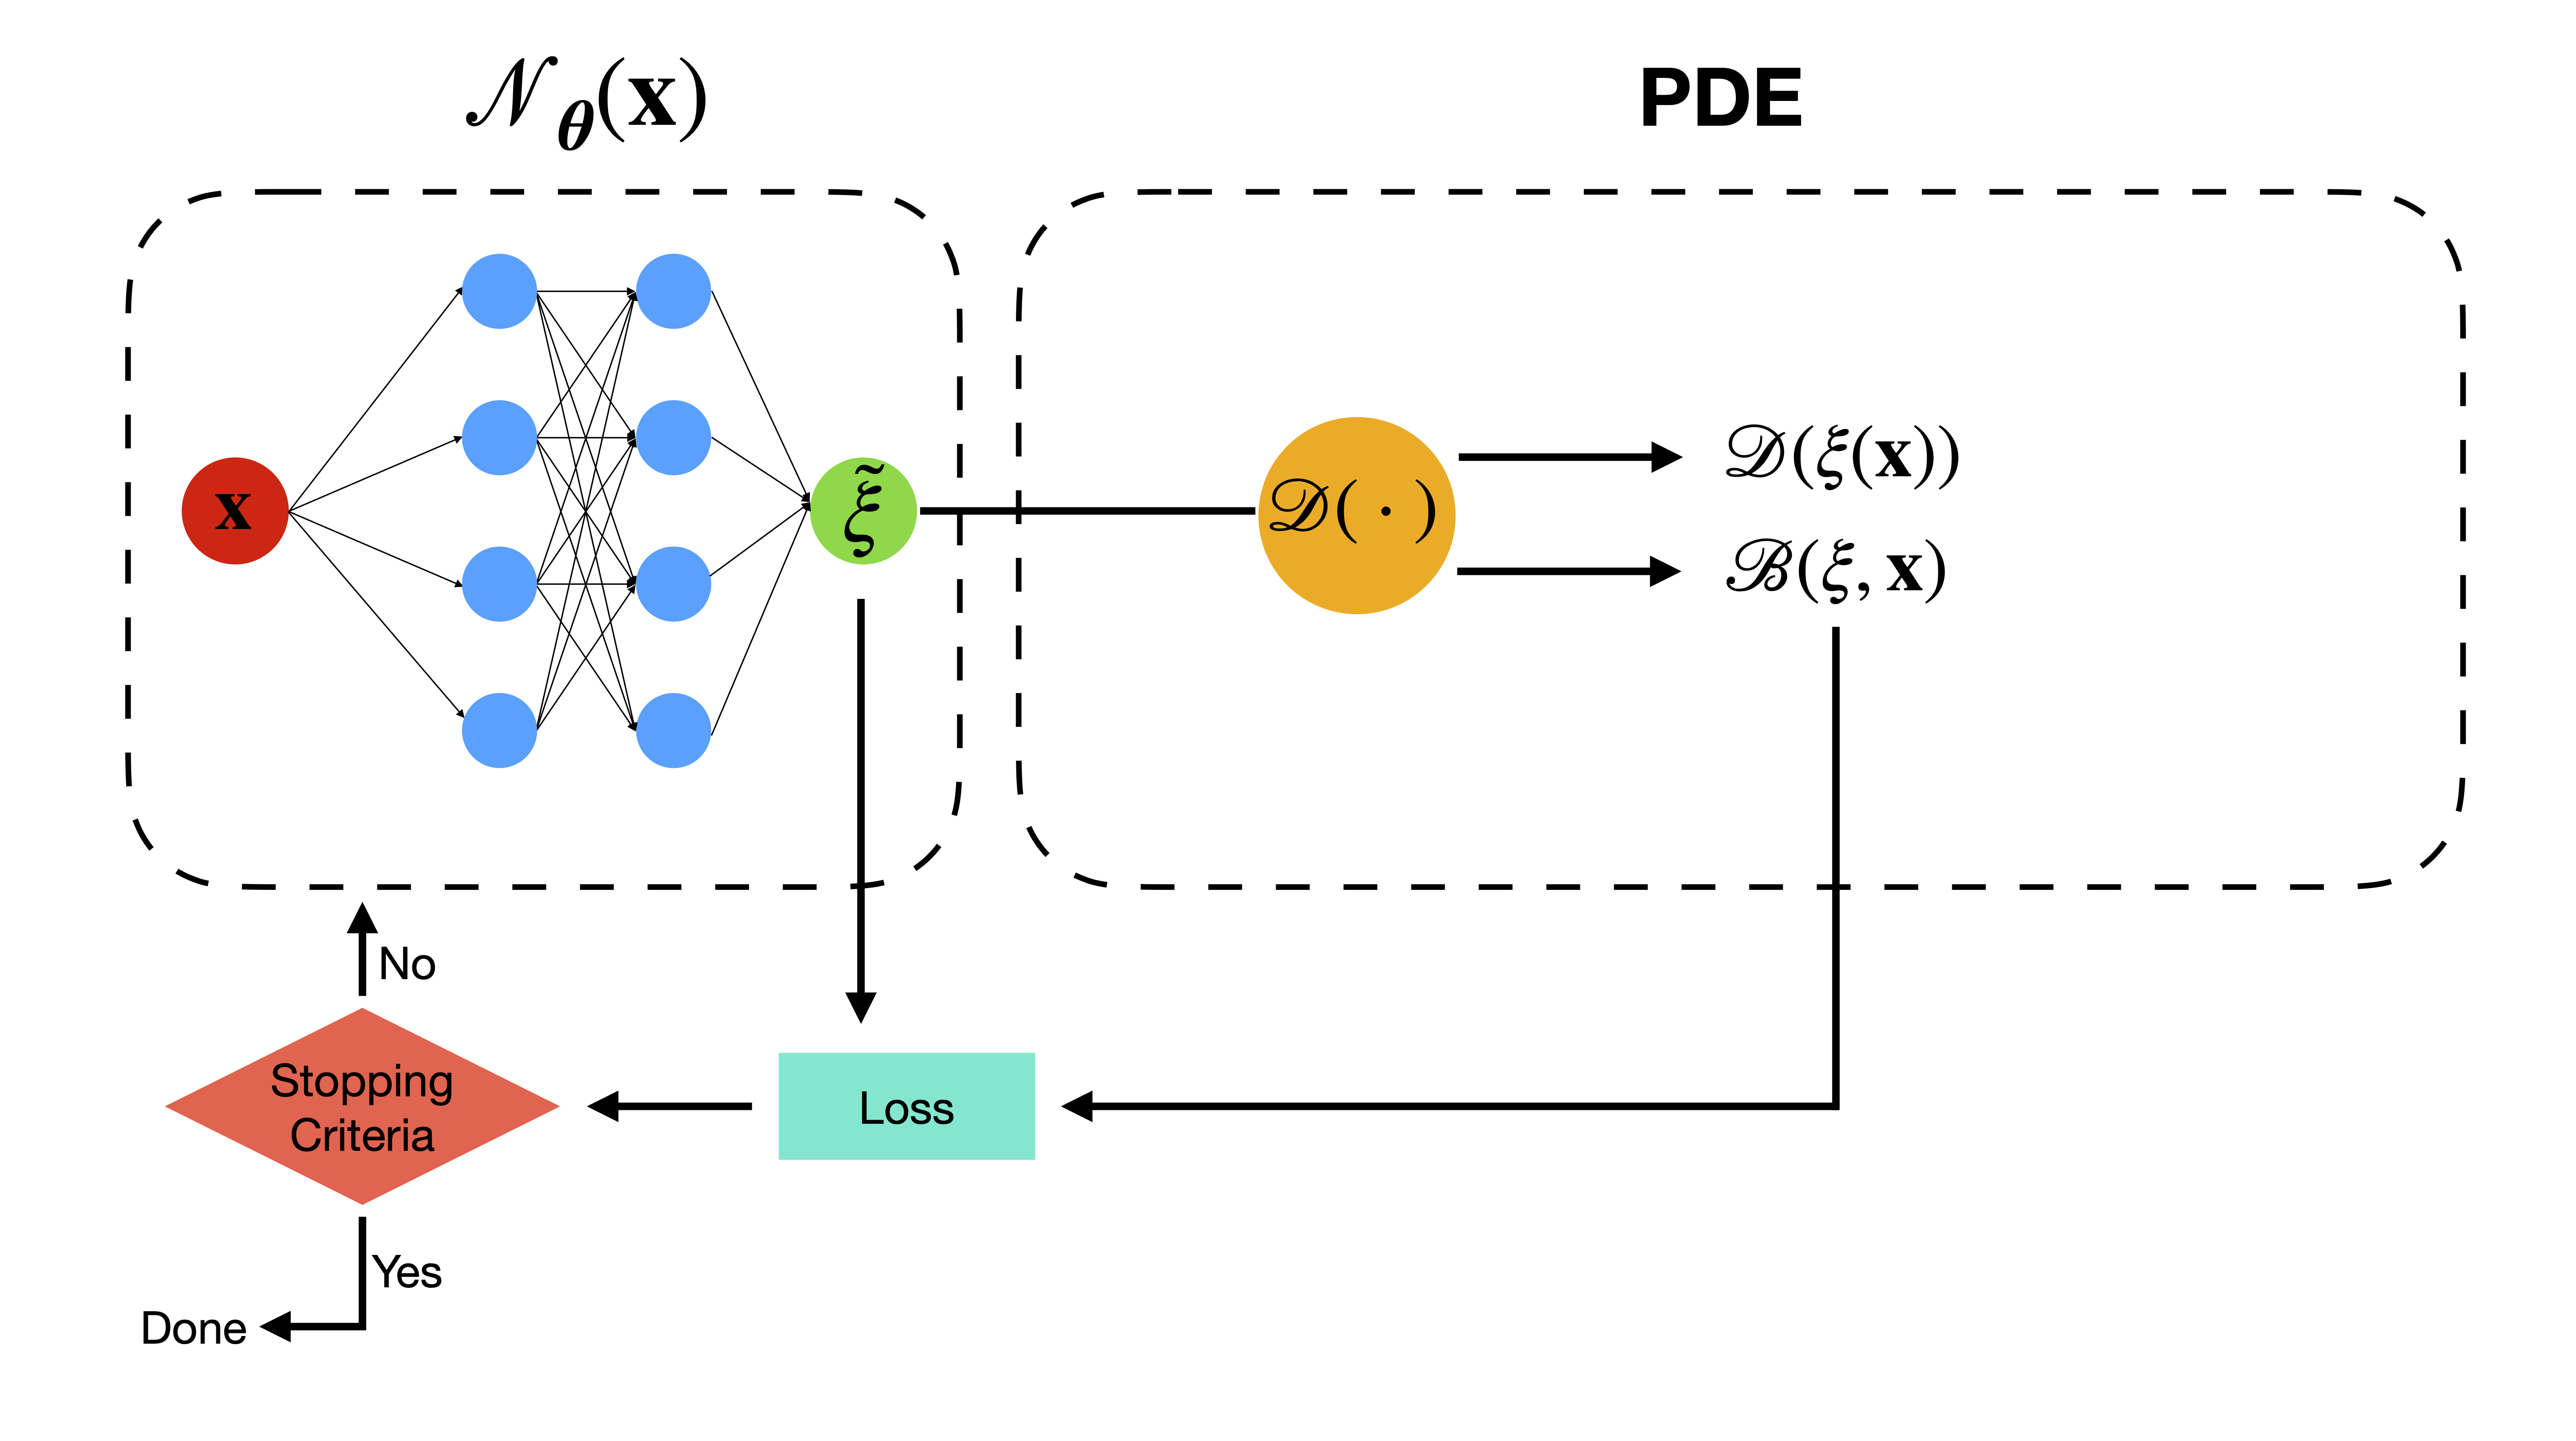
\includegraphics[width=0.9\textwidth]{figures/chap02_preliminaries/pinn.png} 
 \caption{An illustration of a physics informed neural network procedure.}
 \label{fig:pinn}
\end{figure}

Considering an inverse problem, let's rewrite the definition of an abstract PDE \eqref{eqn:abstract_pde} parameterized by $\boldsymbol\gamma$ such that:
\begin{equation}
    \label{eqn:gamma_pde}
    \mathcal{D}(\xi(\mathbf{x});\boldsymbol\gamma)=0 \quad \mathbf{x} \in \Omega.
\end{equation}
Moreover, let's assume we know the solution $\xi(\mathbf{x})$ on some points $\Omega_d \subset \Omega$. In this case, the unknown parameter $\boldsymbol \gamma$ can also be predicted by PINNs just by adding an extra loss term to the loss we defined earlier in a way that 
\begin{equation}
\label{eqn:total_loss}
\begin{split}
       \mathcal{L}(\boldsymbol\theta, \boldsymbol \gamma) &= w_p \frac{1}{|\Omega_p|}\sum_{\mathbf{x} \in \Omega_p} ||\mathcal{D}(\tilde{\xi}(\mathbf{x}); \boldsymbol \gamma)||\\&\quad +w_b \frac{1}{|\partial \Omega_b|}\sum_{\mathbf{x} \in \partial \Omega_b} ||\mathcal{B}(\tilde{\xi},\mathbf{x})||\\&\quad   + w_d \frac{1}{|\Omega_d|}\sum_{\mathbf{x} \in \Omega_d} ||\tilde{\xi}(\mathbf{x})-\xi(x)||,
\end{split}
\end{equation}
where $w_p$, $w_b$, and $w_d$ are the weights of the PDE residual term, boundary term, and data fitting term, respectively. Then, the optimization goal becomes
\begin{equation}
    \label{eqn:optimization}
    \text{finding} \,\, \boldsymbol\theta \,\, and \,\, \boldsymbol\gamma \,\, :     \underset{\boldsymbol\theta,\boldsymbol\gamma}{\arg\min}\,\, \mathcal{L}(\boldsymbol\theta,\boldsymbol\gamma). 
\end{equation}
\chapter{INTRODUCTION}
\label{chap:intro}



\section{Theory}
\label{sec:theory}

The residual of the eikonal equation in a 2D domain ($\Omega$) can be written as
\begin{equation}
    \label{eqn:eik_res}
    r(\boldsymbol{x}):= \sqrt{\nabla T(\boldsymbol{x})\cdot\nabla T(\boldsymbol{x} )}-S(\boldsymbol{x}) = 0, \quad \boldsymbol{x} \in \Omega, 
\end{equation}
where $S(\boldsymbol{x})$ is the slowness which is the reciprocal of the velocity field $V(\boldsymbol{x})$. 

I use two separate ANNs composed of non-linear functions to approximate traveltimes $T(\boldsymbol{x})$ and velocities $V(\boldsymbol{x})$ in the eikonal equation, such that
\begin{equation}
\begin{aligned}
    \label{eqn:network_approx}
     \tilde{T}(\boldsymbol{x}) = \mathcal{N_{T}}(x_{s},\boldsymbol{x};w_{T},b_{T}), \\
     \tilde{V}(\boldsymbol{x}) = \mathcal{N_{V}}(\boldsymbol{x};w_{V},b_{V}),
\end{aligned}     
\end{equation}

where $\mathcal{N_{T}}$ and $\mathcal{N_{V}}$ are the feed-forward neural networks for traveltime and velocity respectively. Here the trainable parameters are weights and biases shown as $w_{T}$ and $b_{T}$ for traveltime NN and $w_{V}$ and $b_{V}$ for velocity NN. To honor multiple shots on the surface, horizontal coordinates of the source location denoted as $x_{s}$, are used as an additional input to the traveltime network, contrary to the velocity network. 

For stability as well as ensuring the solutions remain positive, sigmoid activation function $\sigma$ is applied for both output of the networks before multiplying them with the maximum expected velocity and traveltime values
\begin{equation}
\begin{aligned}
    \label{eqn:network_approx_sigmoid}
     \tilde{T}(\boldsymbol{x}) = T_{max}\,\, \sigma(\mathcal{N_{T}}(x_{s},\boldsymbol{x};w_{T},b_{T})), \\
     \tilde{V}(\boldsymbol{x}) = V_{max}\,\, \sigma(\mathcal{N_{V}}(\boldsymbol{x};w_{V},b_{V})),
\end{aligned}     
\end{equation}

where $V_{max}$ can be decided considering geology of the medium. Whereas, $T_{max}$ can easily be obtained from the observed times. The same strategy for constraining the PINN solution as strictly positive was previously used for prediction of activation maps in cardiac electrophysiology~\cite{cyphk:20}. Recovering the possible sharp transitions in the velocity solution, I also add isotropic total variation regularizer (TV) to the problem. Thus, the composite loss function to train both networks concurrently reads 

\begin{equation}
\begin{aligned}
    \label{eqn:loss}
     \mathcal{L}(w_{T},b_{T},w_{V},b_{V}) = \frac{1}{N_{S} N_{T}} \sum\limits_{n=1}^{N_{S}} \sum\limits_{i=1}^{N_{T}} (\tilde{T}(\boldsymbol{x}_{n,i}) - T_{n,i})^2 \\ + \frac{1}{N_{S} N_{C}} \sum\limits_{n=1}^{N_{S}} \sum\limits_{i=1}^{N_{C}}(\sqrt{\nabla\tilde{T}(\boldsymbol{x}_{n,i}) \cdot\nabla\tilde{T}(\boldsymbol{x}_{n,i})} - \tilde{S}(\boldsymbol{x}_{n,i}))^2 \\ +
     \lambda \frac{1}{N_{C}}\sum\limits_{i=1}^{N_{C}}\norm{\nabla\tilde{V}\boldsymbol({x}_{i})}.
\end{aligned}     
\end{equation}

The first term measures the misfit between the observed traveltimes and the network predicted ones on the receiver positions for each source location. $N_{S}$ denotes the total number of shots and $N_{T}$ represents the number of receivers for a shot. The second term is the eikonal residual computed at the selected collocation points, shown as $N_{C}$, in the computational domain. The third term, on the other hand, introduces TV to the problem. The impact of it controlled by the parameter $\lambda$. \figref{fig:pinn_schematic} illustrates the PINN based inversion schematic which is used in this thesis.

\begin{figure}
 \centering
 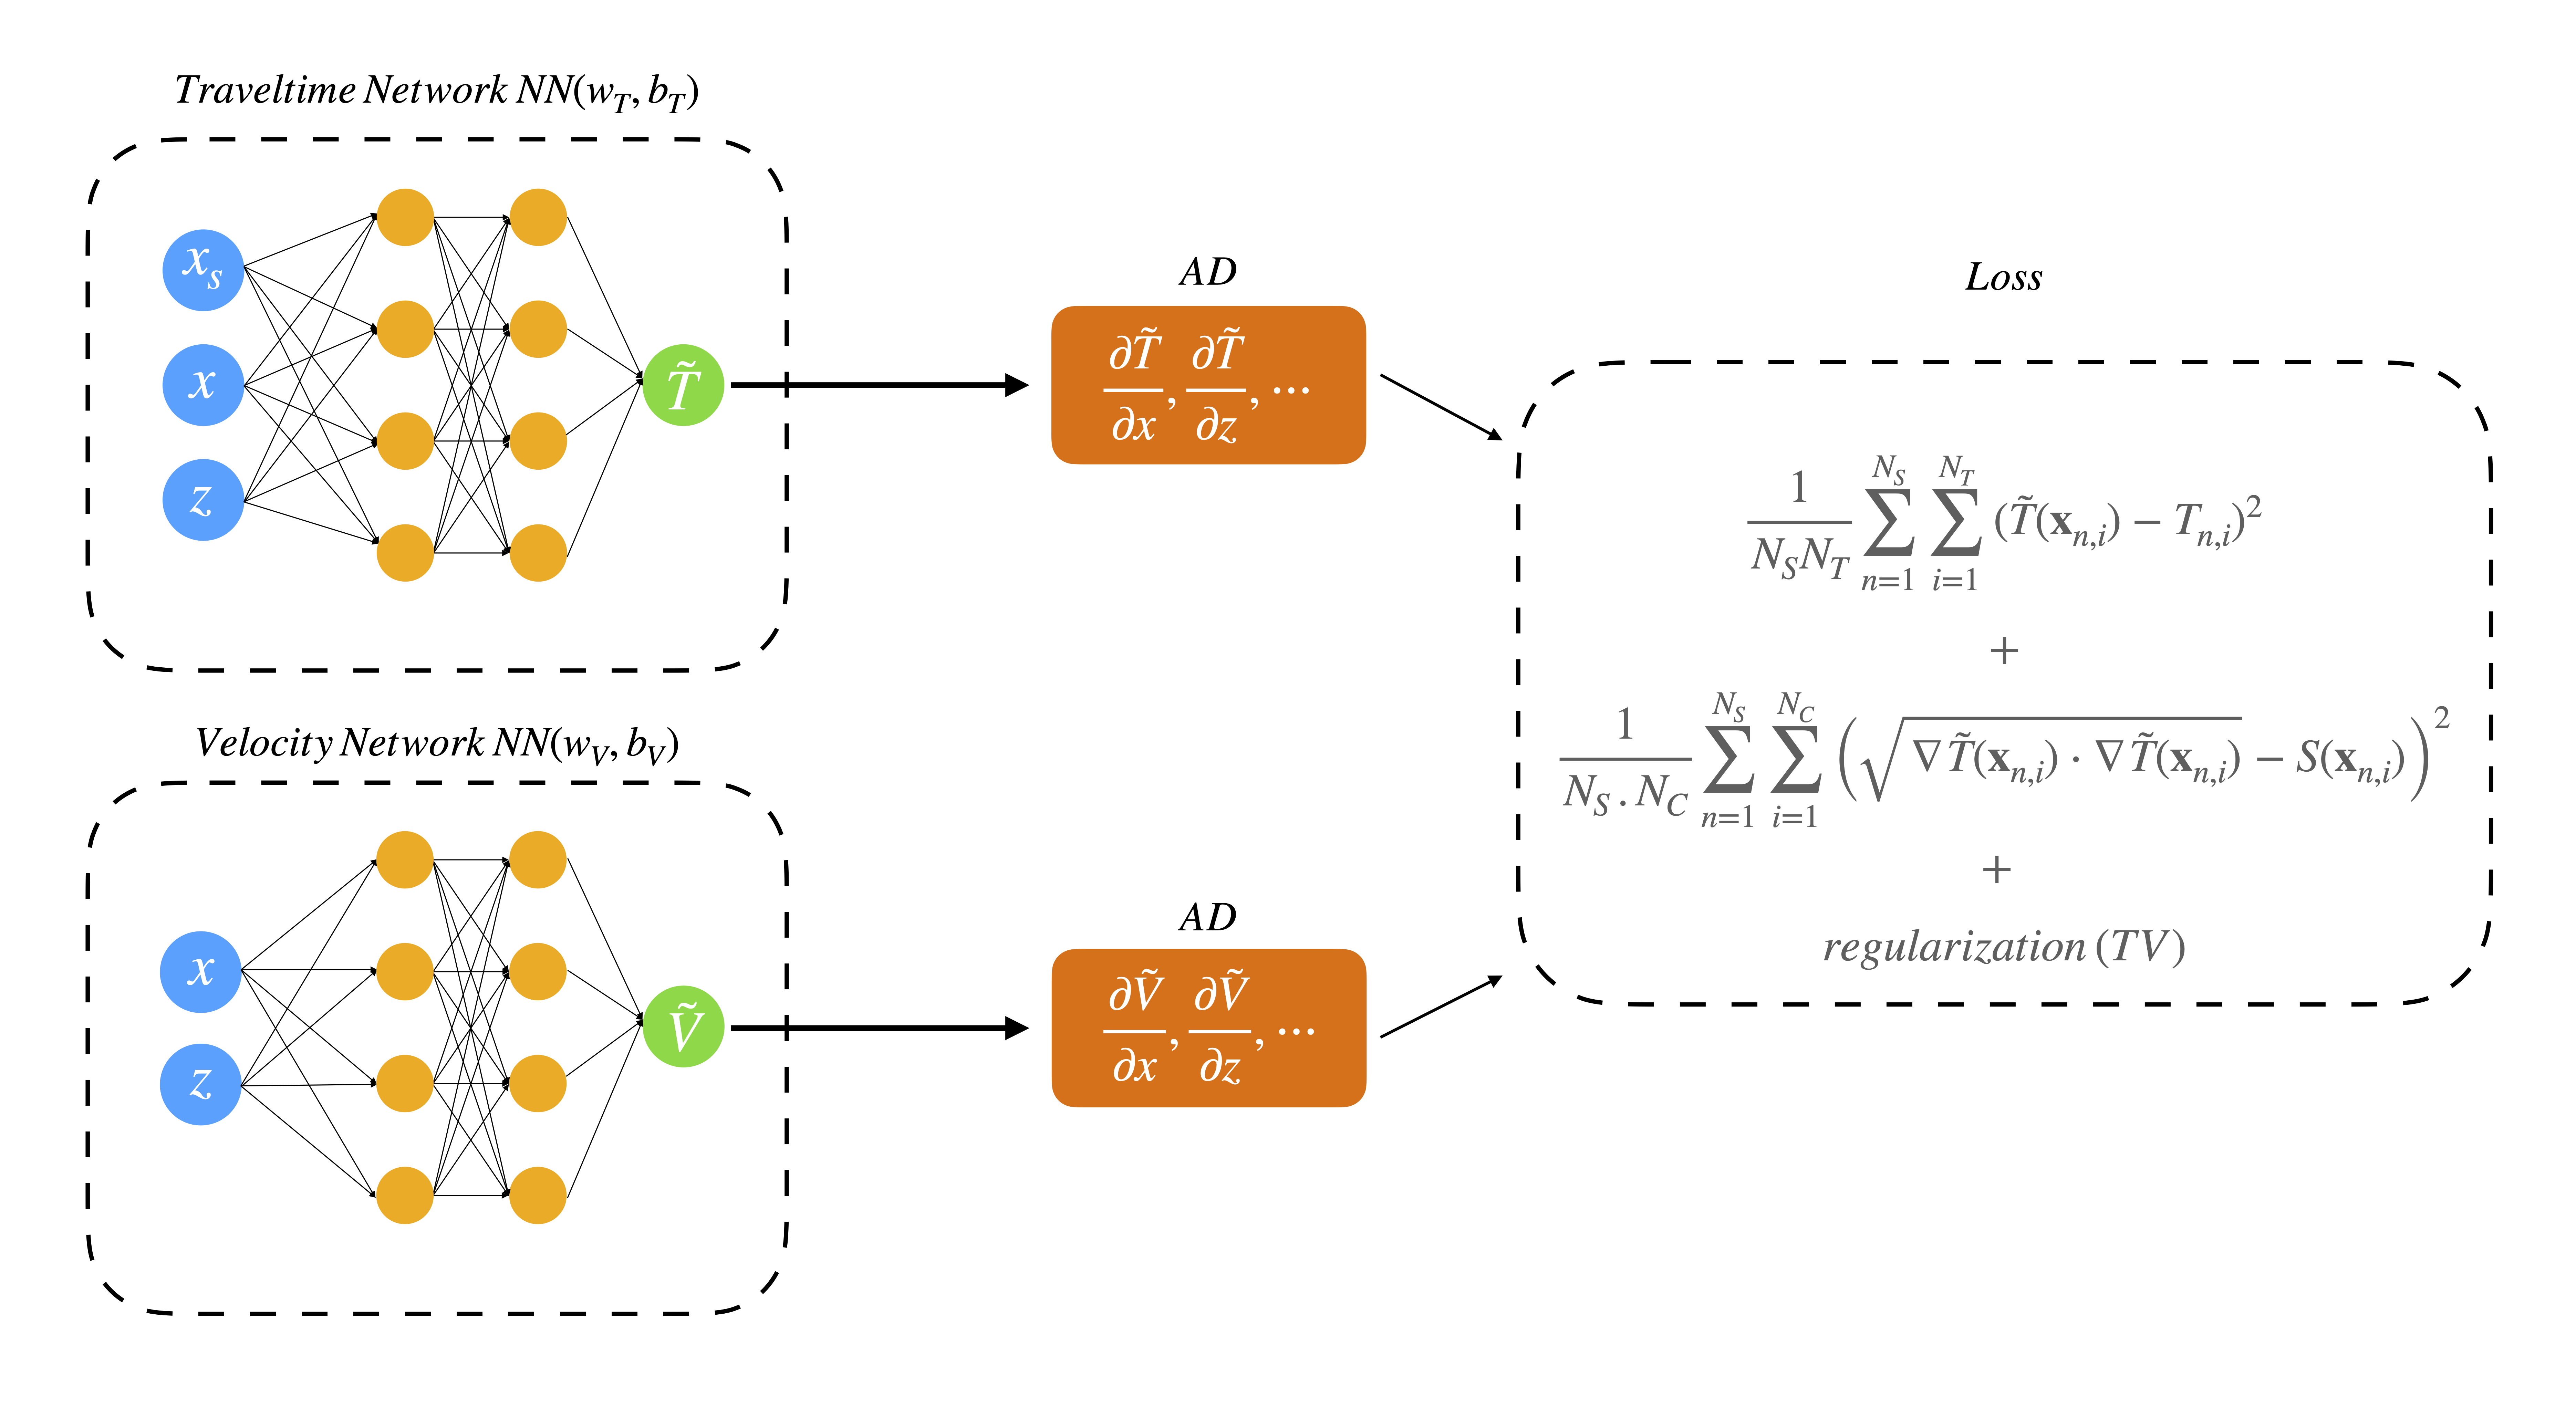
\includegraphics[width=0.9\textwidth]{figures/chap03_pinn_enabled/pinn_schematic} 
 \caption{Illustration of the PINN framework solving for traveltime tomography problem. Two neural networks are used to approximate the traveltime and the velocity. The automatic differentiation is used to calculate the derivatives used in the loss function. Training is performed with a loss function containing the term that minimizes the residuals of the observed times and the network estimated ones, residual of the eikonal equation, and the regularization term.}
 \label{fig:pinn_schematic}
\end{figure}

Hence, the optimization problem seeks to find the optimal network parameters $w_{T}$, $b_{T}$, $w_{V}$, $b_{V}$ such that
\begin{equation}
    \label{eqn:argmin}
    \underset{(w_{T},b_{T},w_{V},b_{V})}{\arg\min} \mathcal{L}(w_{T},b_{T},w_{V},b_{V}).
\end{equation}
\section{Numerical Implementation}
\label{sec:numerical_imp}

First, I test the proposed PINN tomography framework on synthetic examples and then compare the results with the traditional gradient-based traveltime tomography. All PINN enabled tomography implementations are conducted in TensorFlow. For the training, ADAM optimizer~\cite{kb:14} with a default learning rate of 0.001 is chosen before switching to the L-BFGS ~\cite{ln:89} method for the sake of accelerating the convergence. In order to save computational time, all training is performed with a minibatch implementation in which the collocation points are randomly selected from the computational domain using a Latin hypercube sampling ~\cite{s:87}.

The first model example representing a near-surface is a three-layered model with minor folds (\figref{fig:folded_model}). The model size is assumed 36 $\times$ 211 and sampled with a uniform spacing of 10 m both vertically and horizontally ($\Delta z = \Delta x = 10 \, m$). To model the traveltimes, I employ the fast marching method. I use 43 shots with a regular interval of 50 m on the surface.  There are 211 receivers for each shot which makes 43$\times$211 observed surface traveltime data for the PINN implementation (\figref{fig:folded_data}).

 
\begin{figure}
       \centering
       \begin{subfigure}[b]{.9\textwidth}
               \centering
               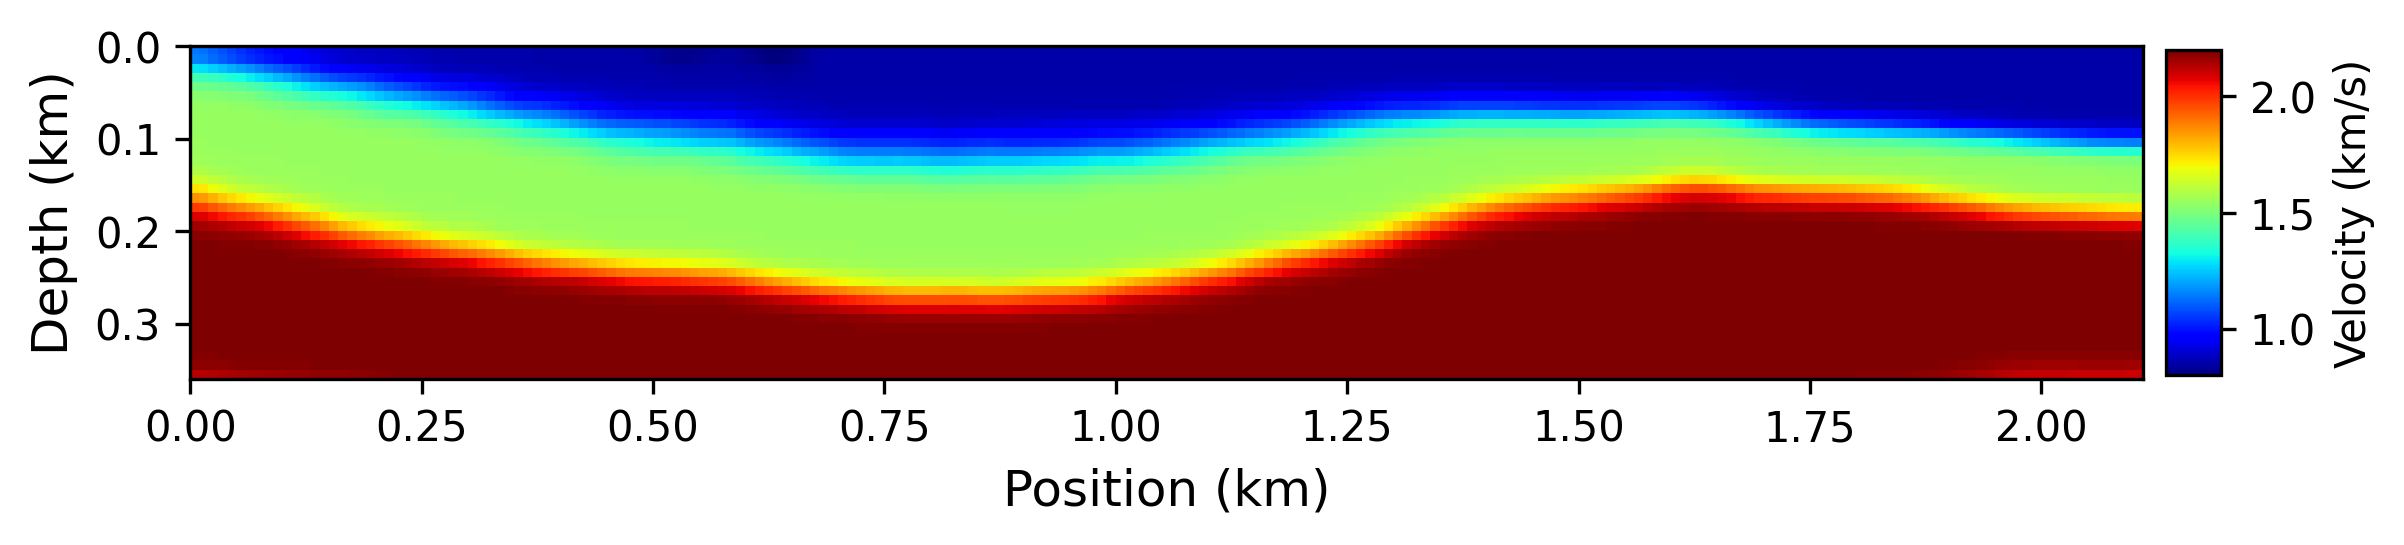
\includegraphics[width=0.9\textwidth]{figures/chap03_pinn_enabled/folded_model} 
               \caption{}
               \label{fig:folded_model}
       \end{subfigure}
       \begin{subfigure}[b]{.9\textwidth}
               \centering
               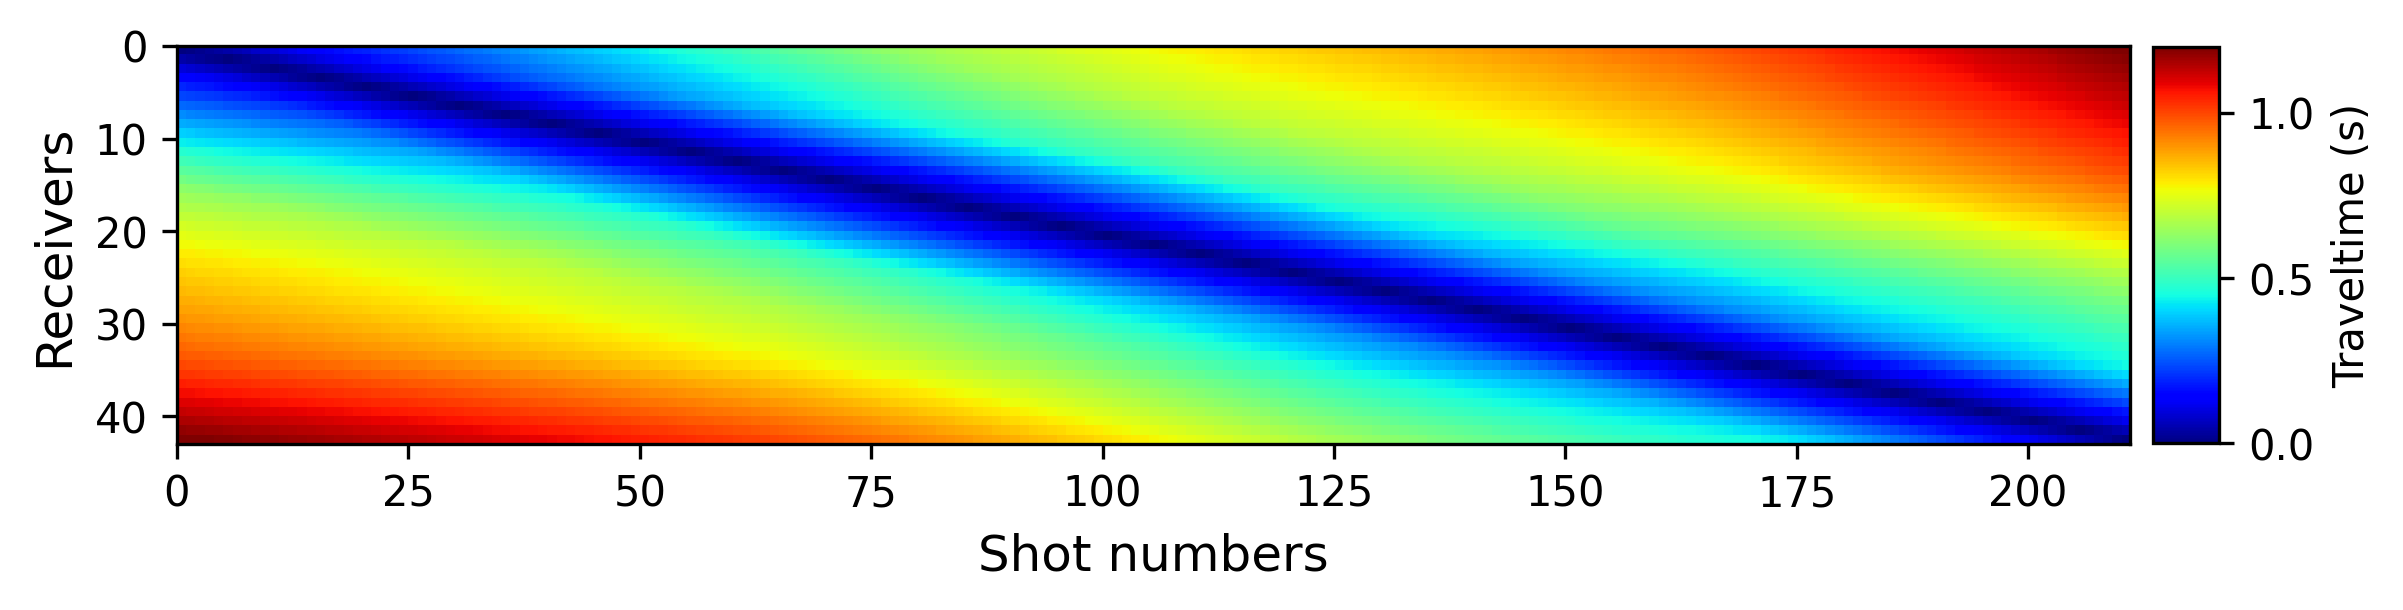
\includegraphics[width=0.9\textwidth]{figures/chap03_pinn_enabled/folded_data}
               \caption{}
               \label{fig:folded_data}
       \end{subfigure}
       \caption{(a) An example of a velocity model for testing the proposed PINN enabled inversion and (b) Image representation of the data aquired from the model. There are 43 shots each having 211 observed traveltimes that are placed in rows to form the image.  }
       \label{fig:folded_example}
\end{figure}


I choose 300 samples from the computational domain with the Latin hypercube sampling method to train the model. After examining the outputs of different settings of the hyperparameters, I use the following tunings: 7 hidden layers with 50 neurons each are used for the traveltime network, while for the velocity, 5 hidden layers with 50 neurons each are decided sufficient as training the velocity network is easier than training the traveltime network. The weight for the TV term is chosen as $\lambda = 10^{-7}$. Moreover, I use $\alpha = 100$ as the weight for the data mismatch term in the loss. Penalizing this specific term during the training helps to improve the accuracy of the retrieved model. The neural network weights are initialized with Xavier initializer~\cite{gb:10}. The estimated velocity model after 20,000 ADAM iterations (\figref{fig:folded_loss_curve}) which is followed by the L-BFGS is shown in \figref{fig:pinn_folded_result}. The retrieved model successfully captures the main features of the true model (\figref{fig:folded_model}). To give a comparison, I additionally perform traditional traveltime tomography using the conjugate-direction (CD) method ~\cite{c:14}. The acquisition geometry is the same as for the PINN tomography and the tomographic inversion is obtained by implementing 10 linearization updates each having 30 conjugate-gradient iterations. The convergence history for the traditional approach is presented in \figref{fig:convergence_curve1}. Starting velocity model for the inversion is obtained by taking the vertical profile from the true model (\figref{fig:folded_model}) and then applying strong smoothing. The inverted model and the initial one is given in \figref{fig:std_tomo1}. Even though the inversion is started with a priori knowledge of the vertical profile from the region, the inversion can not approach the true velocities in many places as the optimization traps in local minimum points.

\begin{figure}
 \centering
 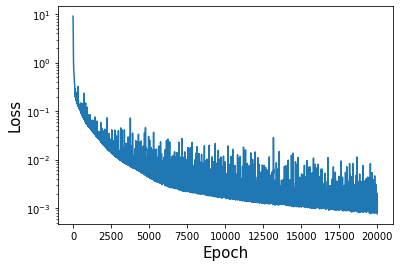
\includegraphics[width=0.7\textwidth]{figures/chap03_pinn_enabled/folded_loss_curve} 
 \caption{Loss curve of the PINN tomography after 20,000 ADAM iterations using minibatch implementation with a batch size of 300.}
 \label{fig:folded_loss_curve}
\end{figure}


\begin{figure}
 \centering
 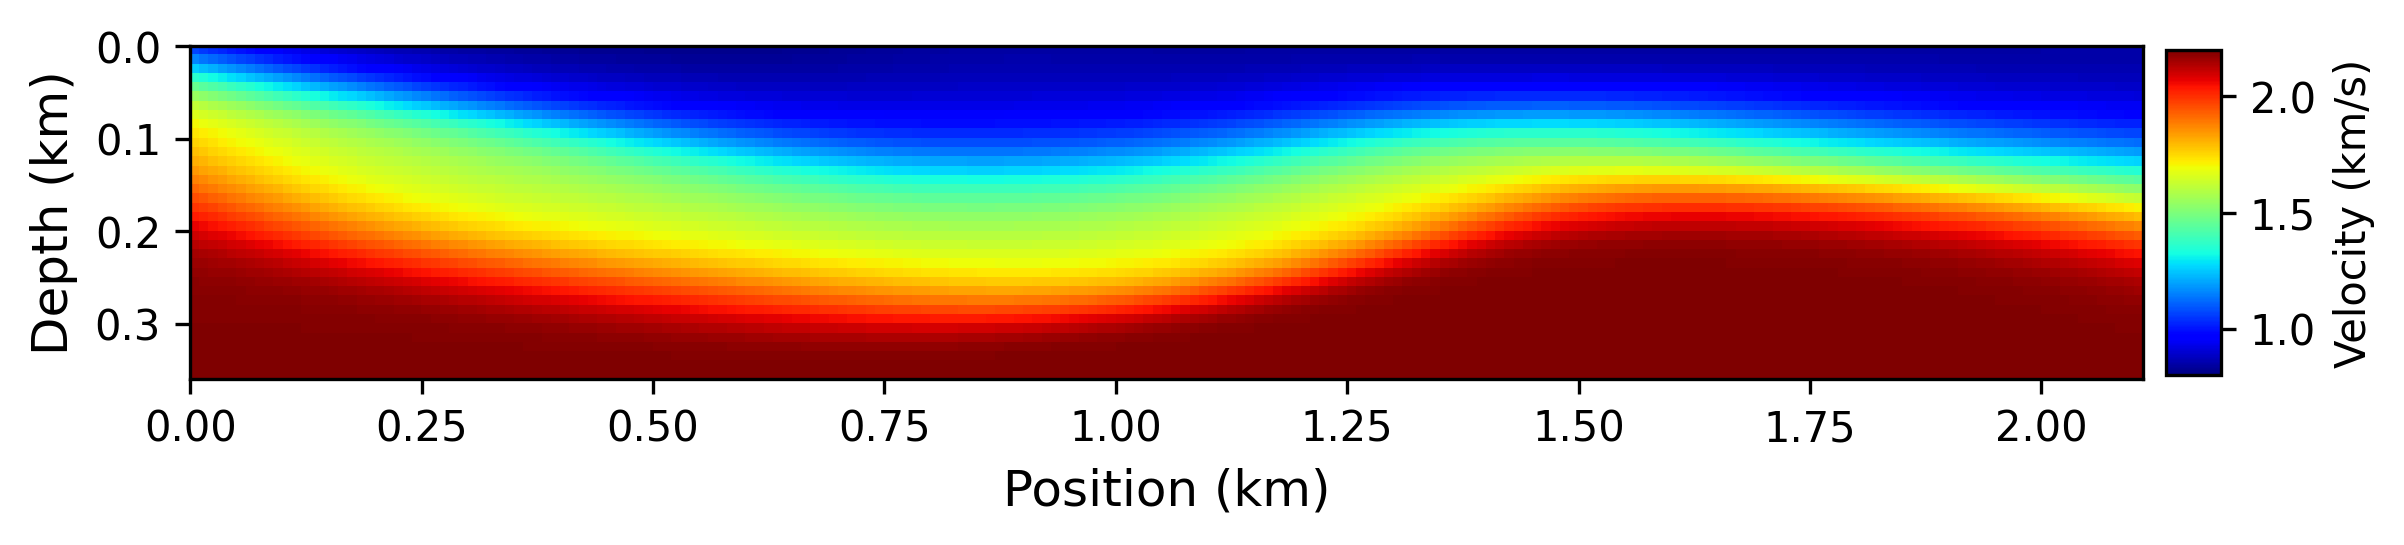
\includegraphics[width=1.0\textwidth]{figures/chap03_pinn_enabled/pinn_folded_result} 
 \caption{PINN predicted velocity model after L-BFGS iterations.}
 \label{fig:pinn_folded_result}
\end{figure}

\begin{figure}
 \centering
 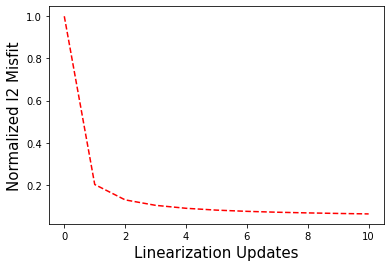
\includegraphics[width=0.7\textwidth]{figures/chap03_pinn_enabled/convergence_curve1} 
 \caption{Convergence history of the gradient-based tomography after 10 linearization updates. 30 conjugate-gradient iterations are used for each linearization.}
 \label{fig:convergence_curve1}
\end{figure}

\begin{figure}
       \centering
       \begin{subfigure}[b]{1.\textwidth}
               \centering
               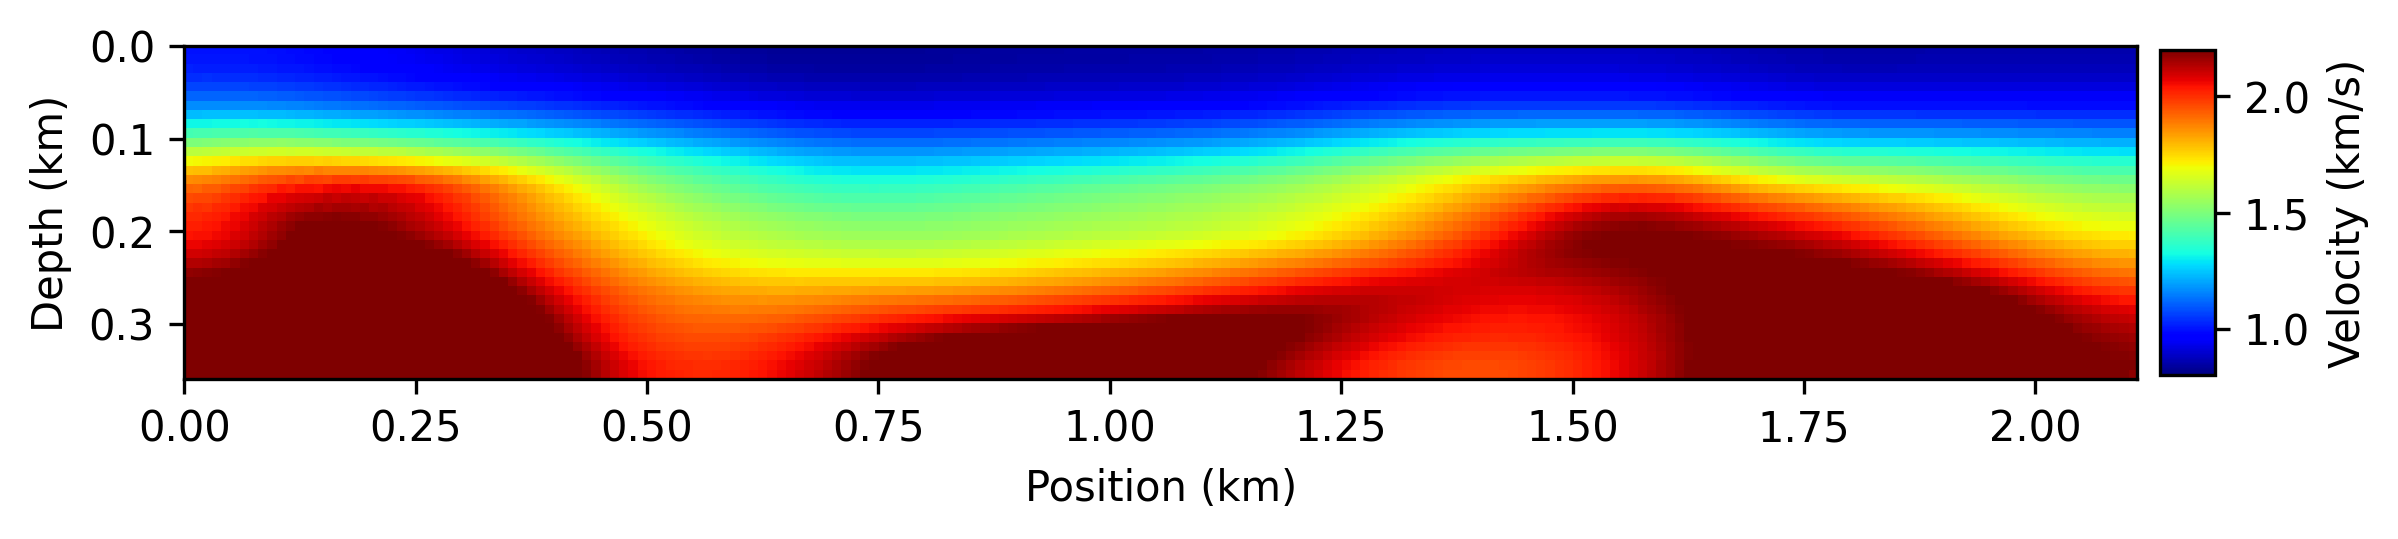
\includegraphics[width=0.9\textwidth]{figures/chap03_pinn_enabled/folded_tomo} 
               \caption{}
               \label{fig:folded_tomo}
       \end{subfigure}
       \begin{subfigure}[b]{1.\textwidth}
               \centering
               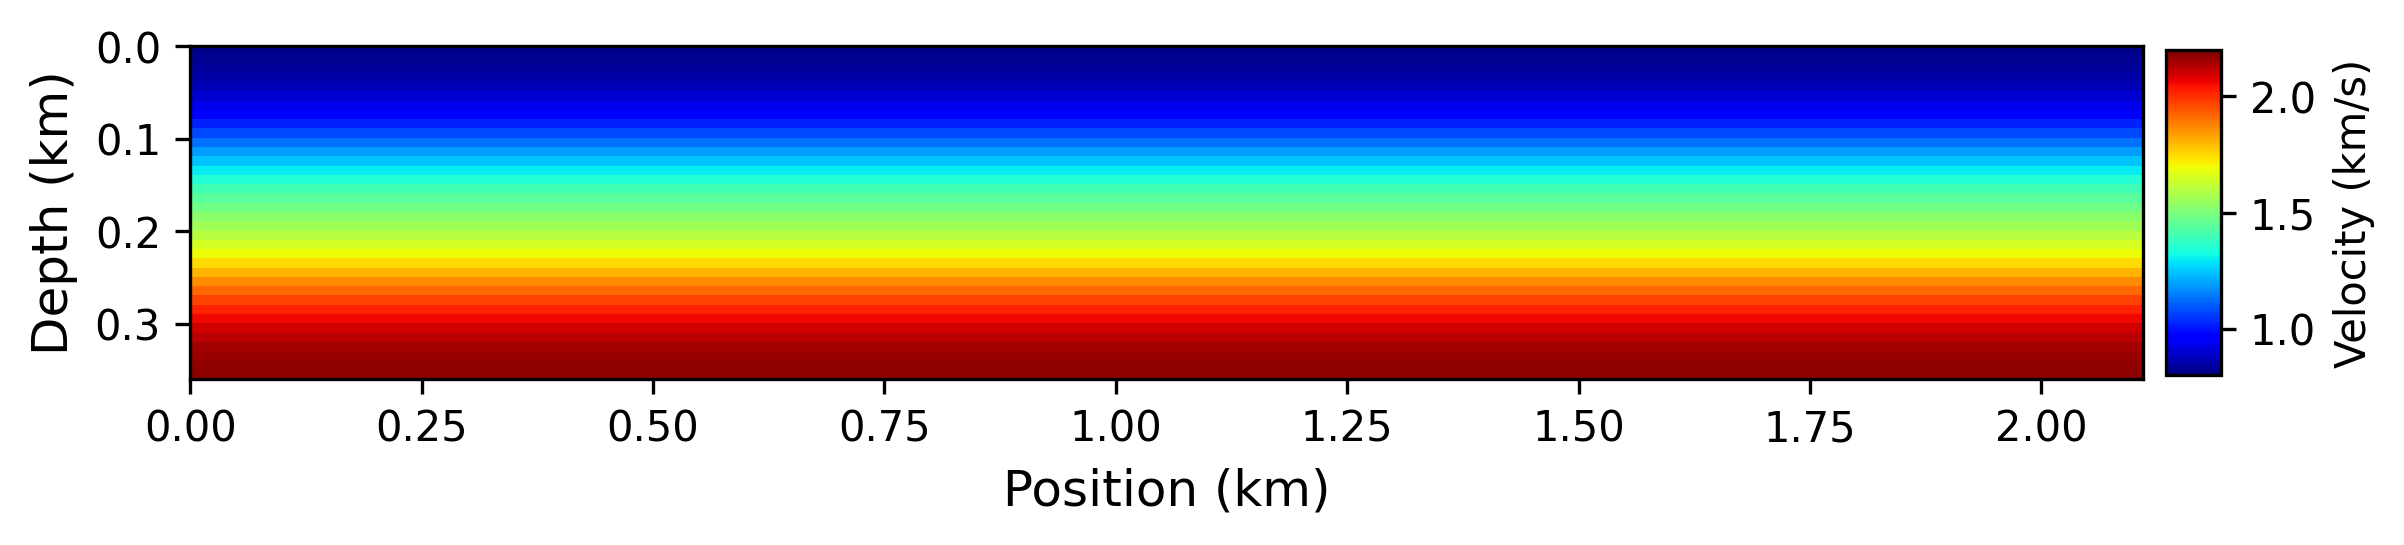
\includegraphics[width=0.9\textwidth]{figures/chap03_pinn_enabled/folded_init}
               \caption{}
               \label{fig:folded_init}
       \end{subfigure}
       \caption{(a) Inverted model from the conventional tomography and (b) Starting velocity model for tomography.}
       \label{fig:std_tomo1}
\end{figure}

The next example for testing the proposed approach is a more complicated near-surface model containing fault systems (\figref{fig:thesis_model2}). The acquisition parameters selected in the first example is again employed for acquiring the data (\figref{fig:thesis_model2_data}). This time, PINN inversion is performed by using 40,000 Adam iterations  (\figref{fig:thesis_model2_loss}) with a minibatch size of 500 and followed by the L-BFGS algorithm. The final inversion result is provided in \figref{fig:thesis_model2_pinn}. Again for comparison, traditional tomography is implemented. No further improvement in the convergence is observed after the 10th linearization step (\figref{fig:convergence_curve2}). Although the inverted model (\figref{fig:model2_tomo}) is generally similar to the predicted model by the PINN  (\figref{fig:thesis_model2_pinn}), it presents wrongly estimated high velocities some of the areas in the model maybe bacause of the contradicting gradient information along the shot dimension. To present a quantitative assessment of the results from both examples, I compare vertical velocity profiles obtained from four different positions (\figref{fig:example_1_profiles}) (\figref{fig:example_2_profiles}) as well as the percent error maps (\figref{fig:error}). As expected from the traveltime tomography, both methods provide a smooth representation of the actual models. However, in deeper parts of the models traditional approach tends to deviate from the true velocities, which is especially observable for the first example. As expected from the traveltime tomography, both methods provide a smooth representation of the actual models. However, in deeper parts of the models traditional approach tends to deviate from the true velocities, which is especially observable for the first example. Also, the percentage velocity errors from the PINN-based approach are generally lower than the errors from the classical method.
\begin{figure}
       \centering
       \begin{subfigure}[b]{.9\textwidth}
               \centering
               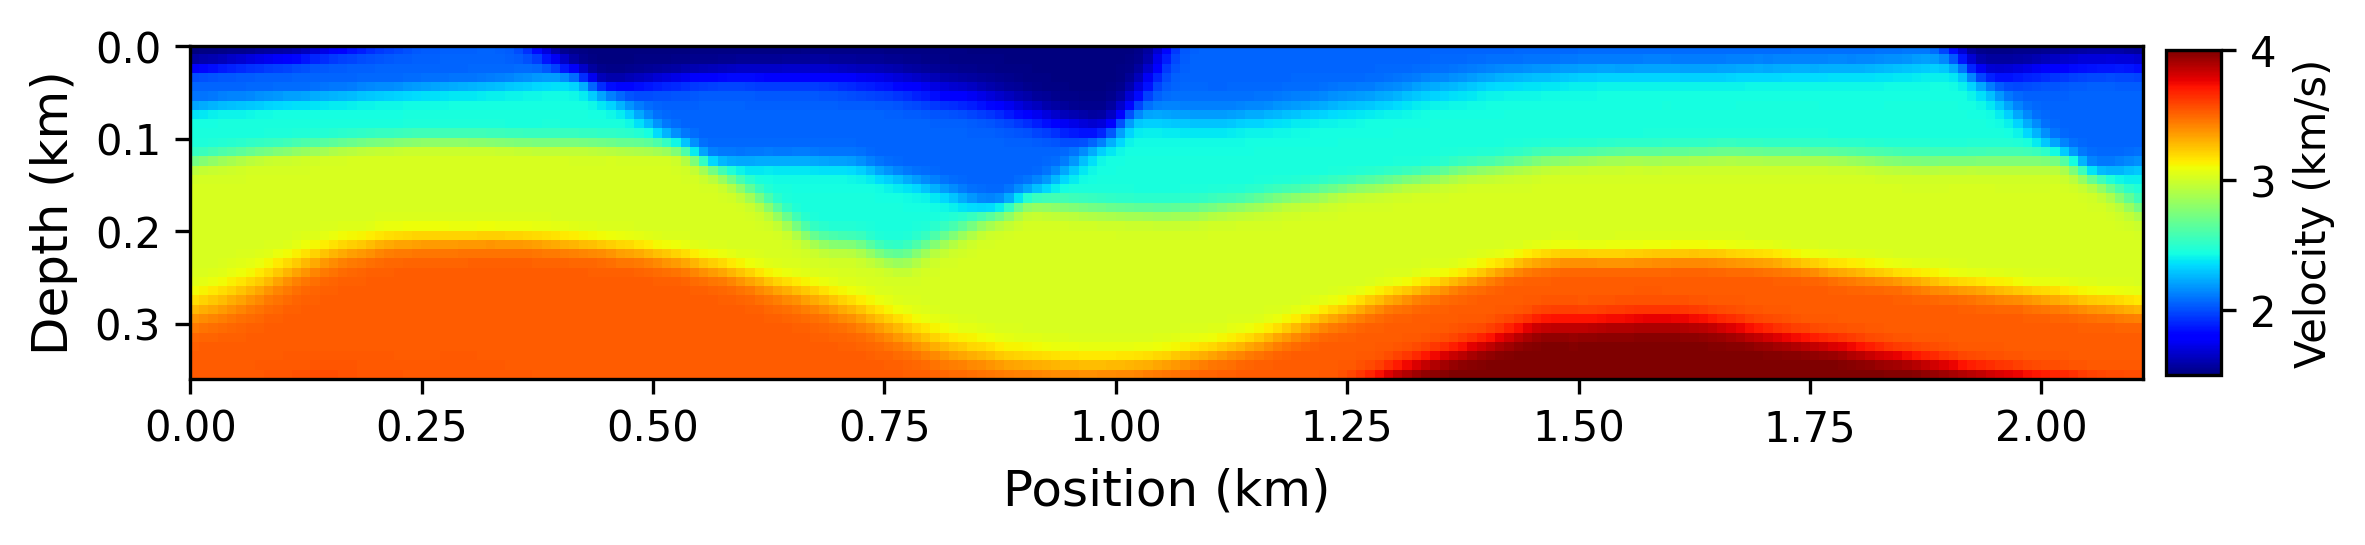
\includegraphics[width=0.9\textwidth]{figures/chap03_pinn_enabled/thesis_model2} 
               \caption{}
               \label{fig:thesis_model2}
       \end{subfigure}
       \begin{subfigure}[b]{.9\textwidth}
               \centering
               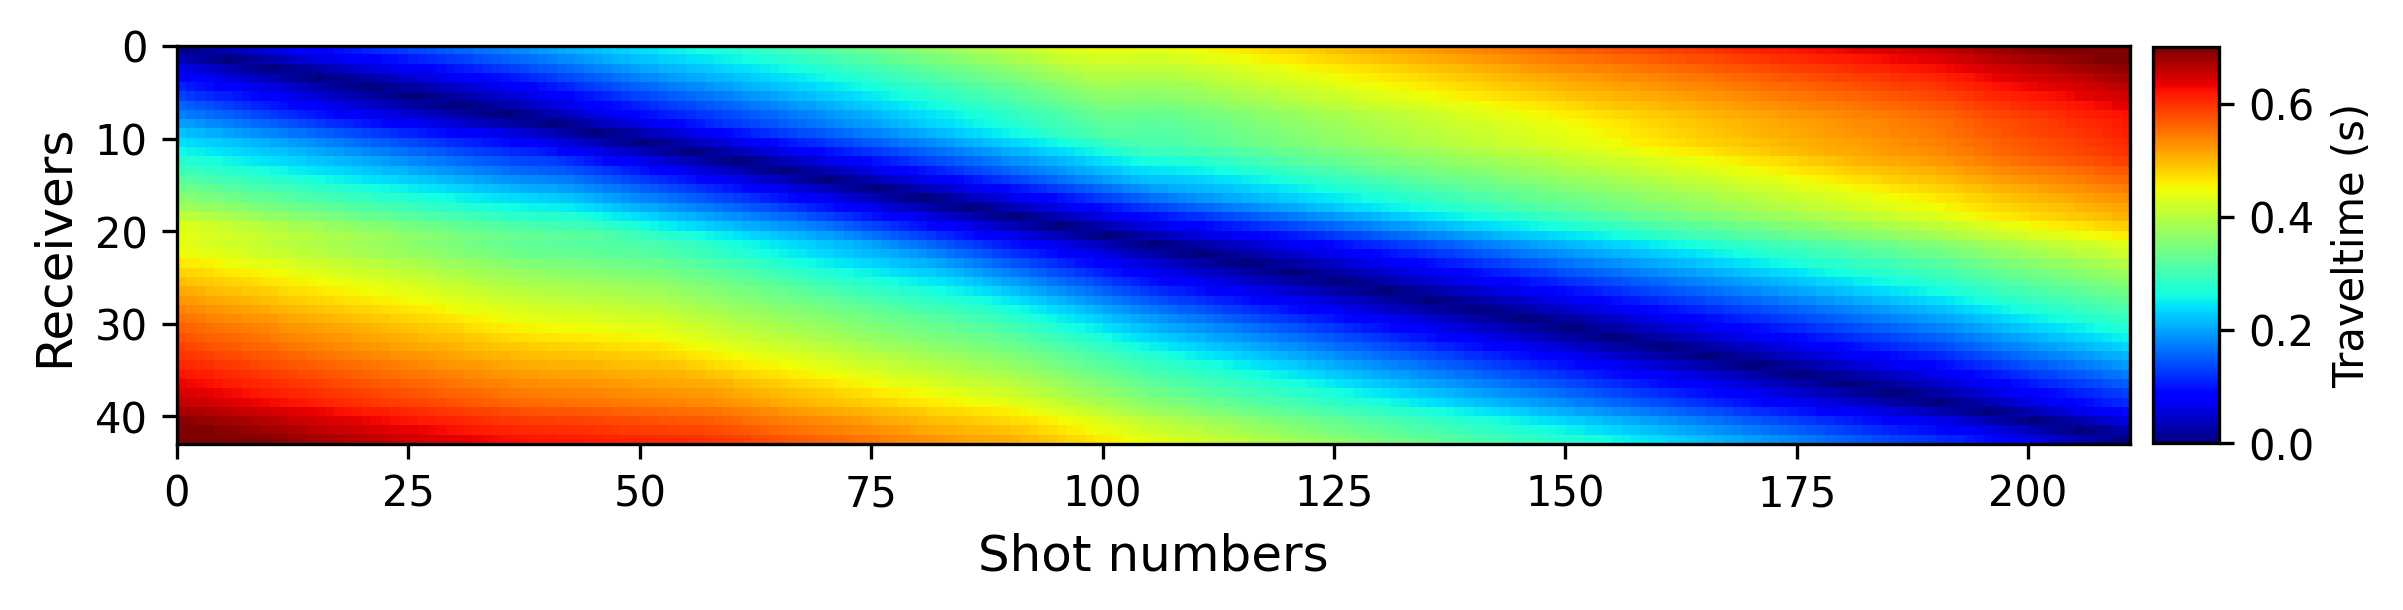
\includegraphics[width=0.9\textwidth]{figures/chap03_pinn_enabled/thesis_model2_data}
               \caption{}
               \label{fig:thesis_model2_data}
       \end{subfigure}
       \caption{(a) An example of a velocity model for testing the proposed PINN enabled inversion and (b) Image representation of the data aquired from the model. There are 43 shots each having 211 observed traveltimes that are placed in rows to form the image.  }
       \label{fig:model2}
\end{figure}

\begin{figure}
 \centering
 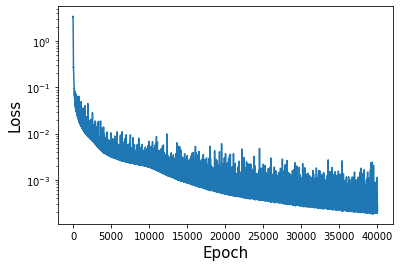
\includegraphics[width=0.7\textwidth]{figures/chap03_pinn_enabled/thesis_model2_loss} 
 \caption{Loss curve of the PINN tomography after 40,000 ADAM iterations using minibatch implementation with a batch size of 500.}
 \label{fig:thesis_model2_loss}
\end{figure}

\begin{figure}
 \centering
 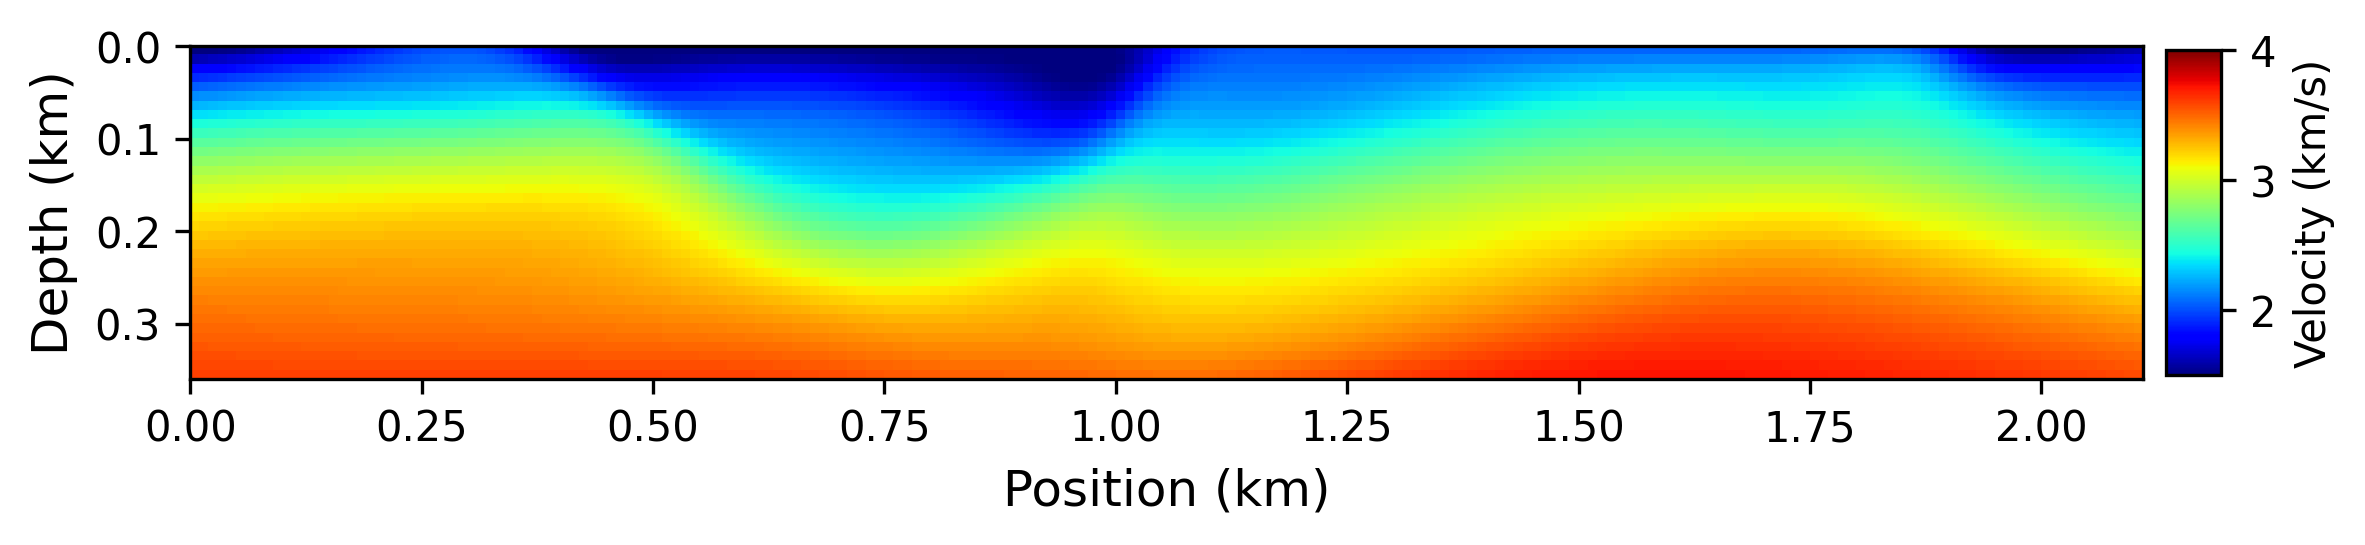
\includegraphics[width=1.0\textwidth]{figures/chap03_pinn_enabled/thesis_model2_pinn} 
 \caption{PINN predicted velocity model after L-BFGS iterations.}
 \label{fig:thesis_model2_pinn}
\end{figure}

\begin{figure}
 \centering
 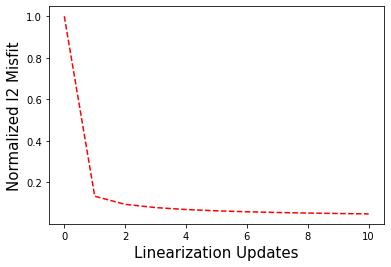
\includegraphics[width=0.7\textwidth]{figures/chap03_pinn_enabled/convergence_curve2} 
 \caption{Convergence history of the gradient-based tomography after 10 linearization updates. 30 conjugate-gradient iterations are used for each linearization.}
 \label{fig:convergence_curve2}
\end{figure}

\begin{figure}
       \centering
       \begin{subfigure}[b]{1.\textwidth}
               \centering
               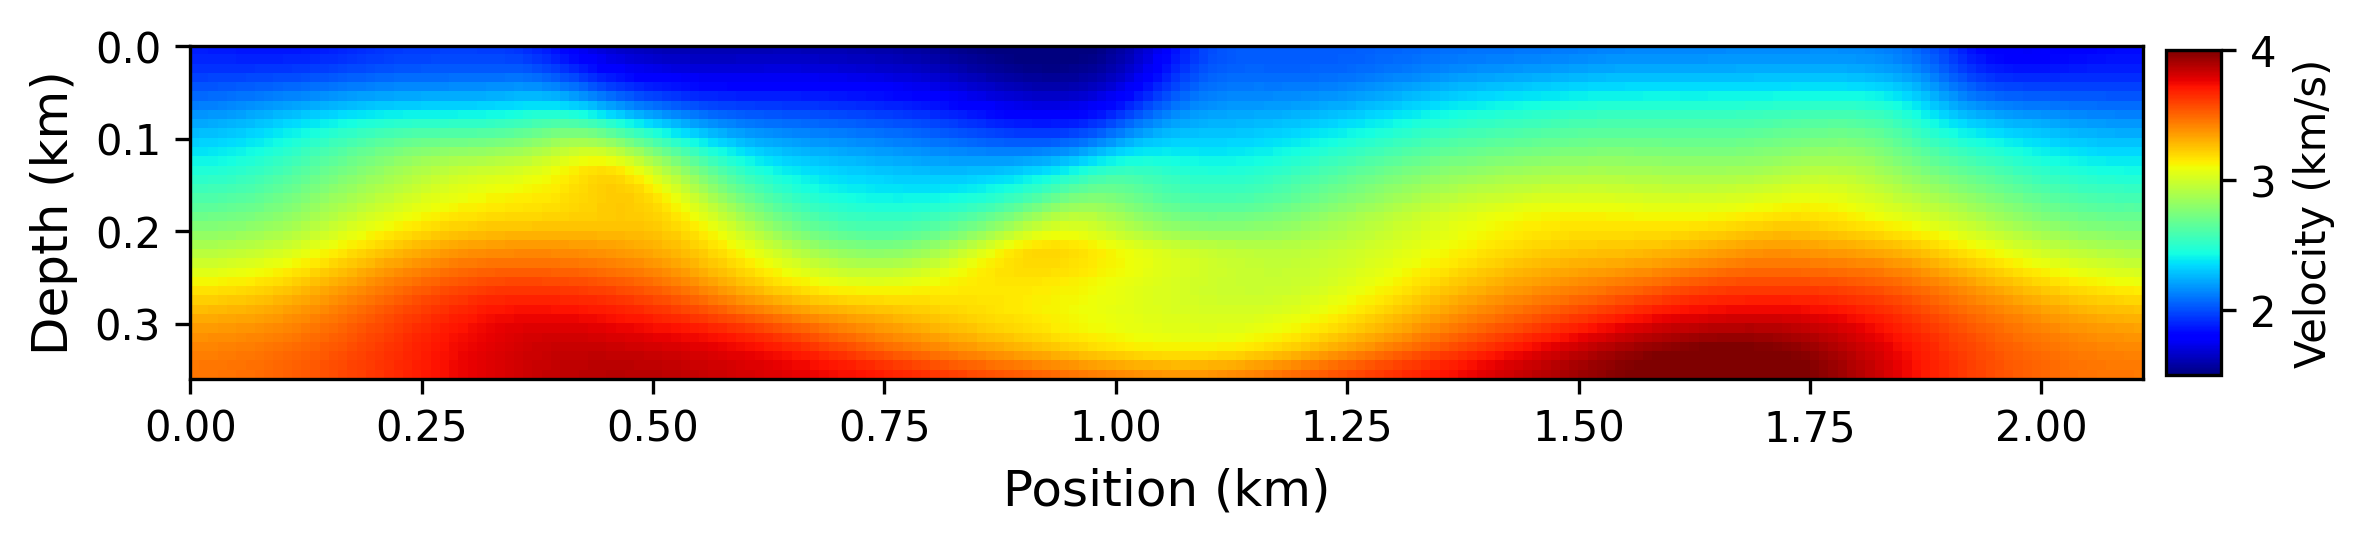
\includegraphics[width=0.9\textwidth]{figures/chap03_pinn_enabled/model2_tomo} 
               \caption{}
               \label{fig:model2_tomo}
       \end{subfigure}
       \begin{subfigure}[b]{1.\textwidth}
               \centering
               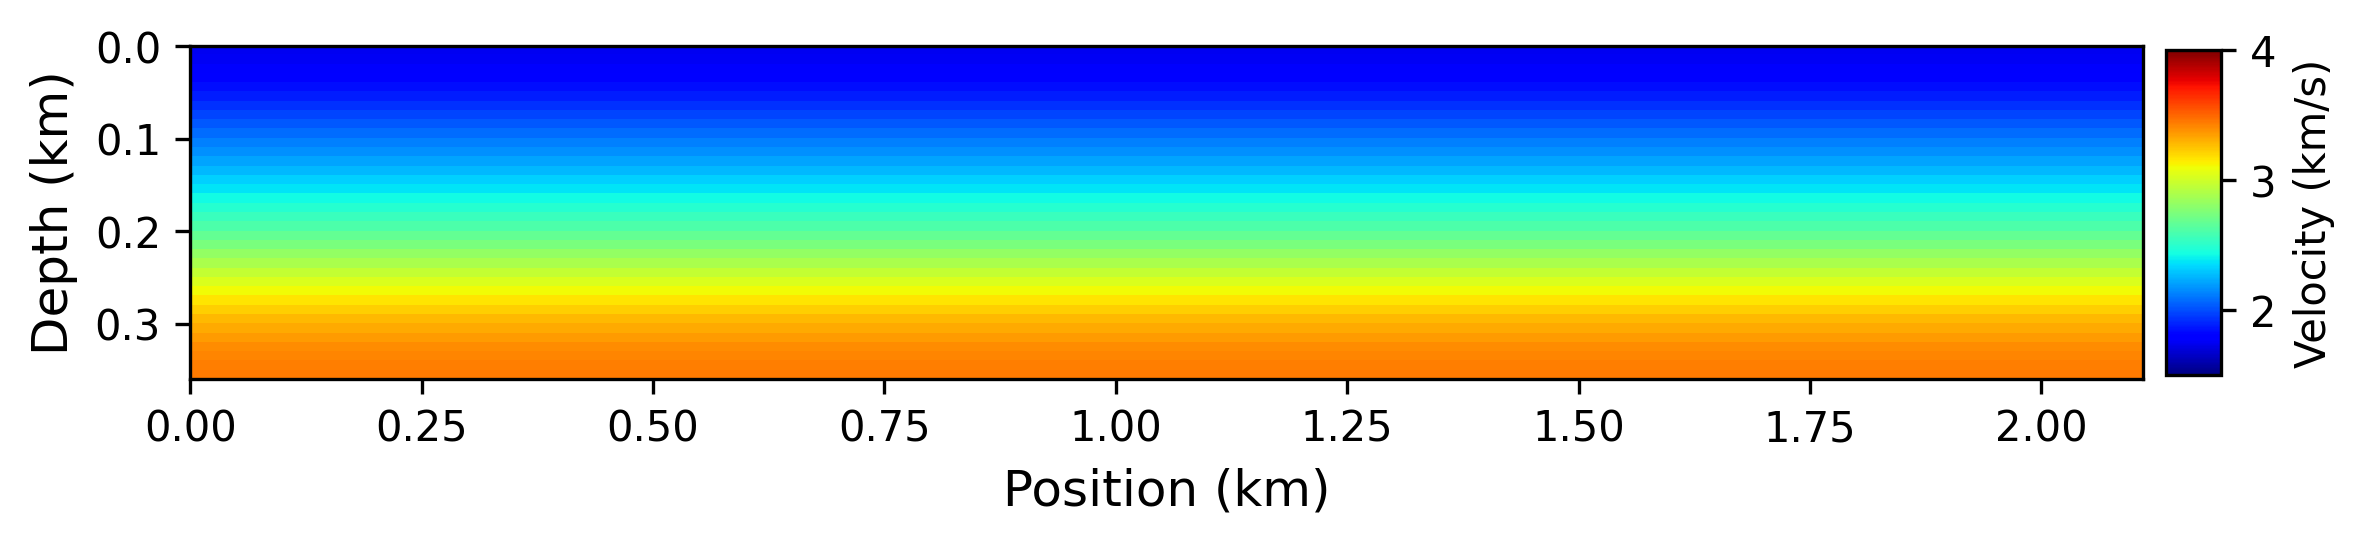
\includegraphics[width=0.9\textwidth]{figures/chap03_pinn_enabled/model2_init}
               \caption{}
               \label{fig:model2_init}
       \end{subfigure}
       \caption{(a) Inverted model from the conventional tomography and (b) Starting velocity model for tomography.}
       \label{fig:std_tomo2}
\end{figure}

\begin{figure}
 \centering
 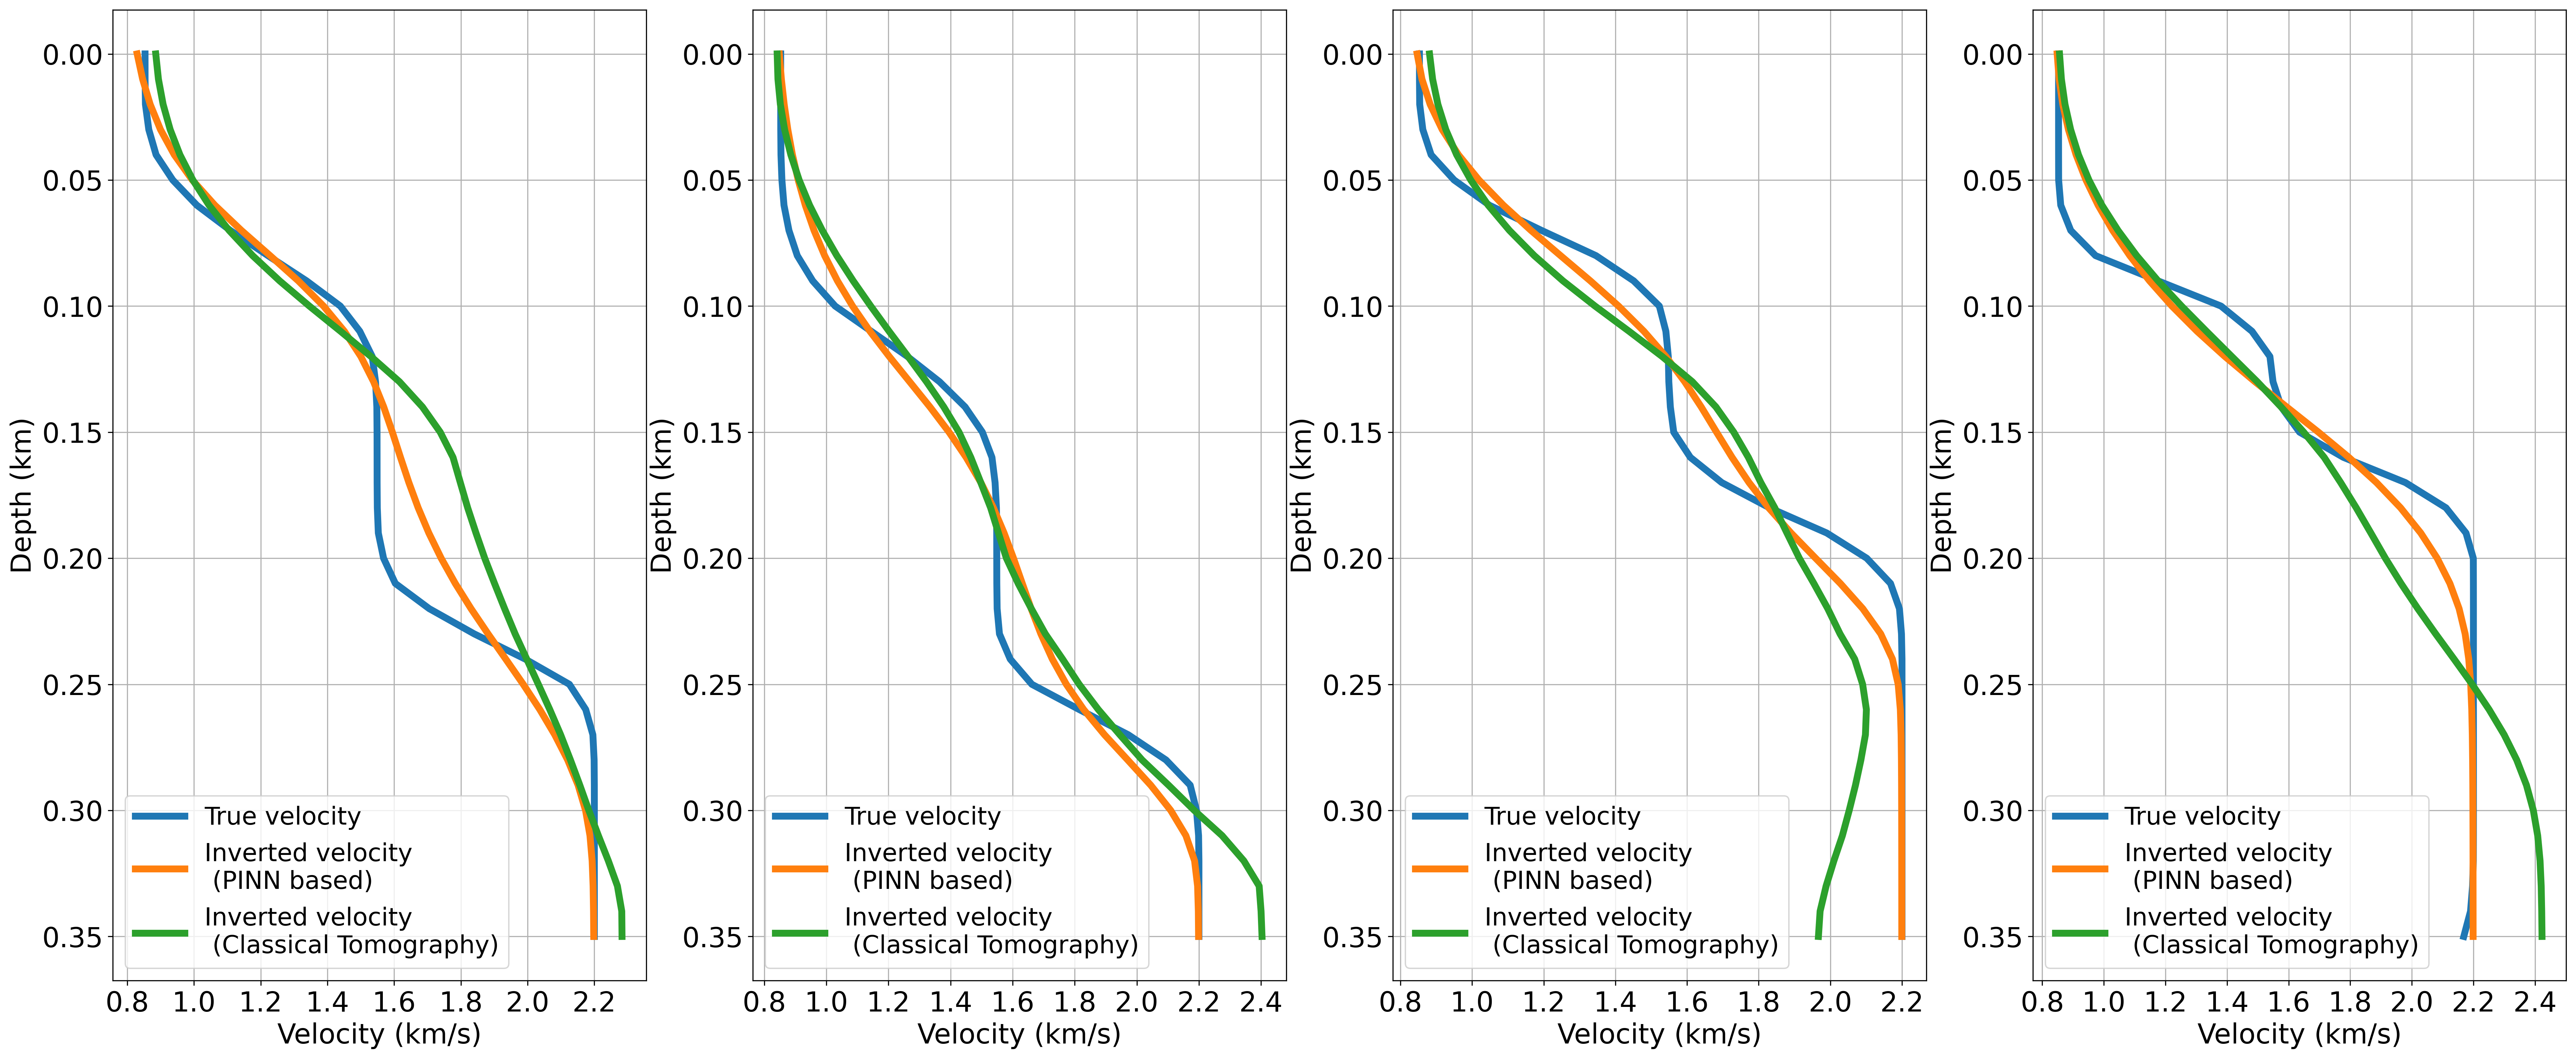
\includegraphics[width=0.9\textwidth]{figures/chap03_pinn_enabled/example_1_profiles} 
 \caption{Vertical velocity profiles at 0.4 km, 0.9 km, 1.3 km and 1.9 km from left to right respectively for the first example.}
 \label{fig:example_1_profiles}
\end{figure}

\begin{figure}
 \centering
 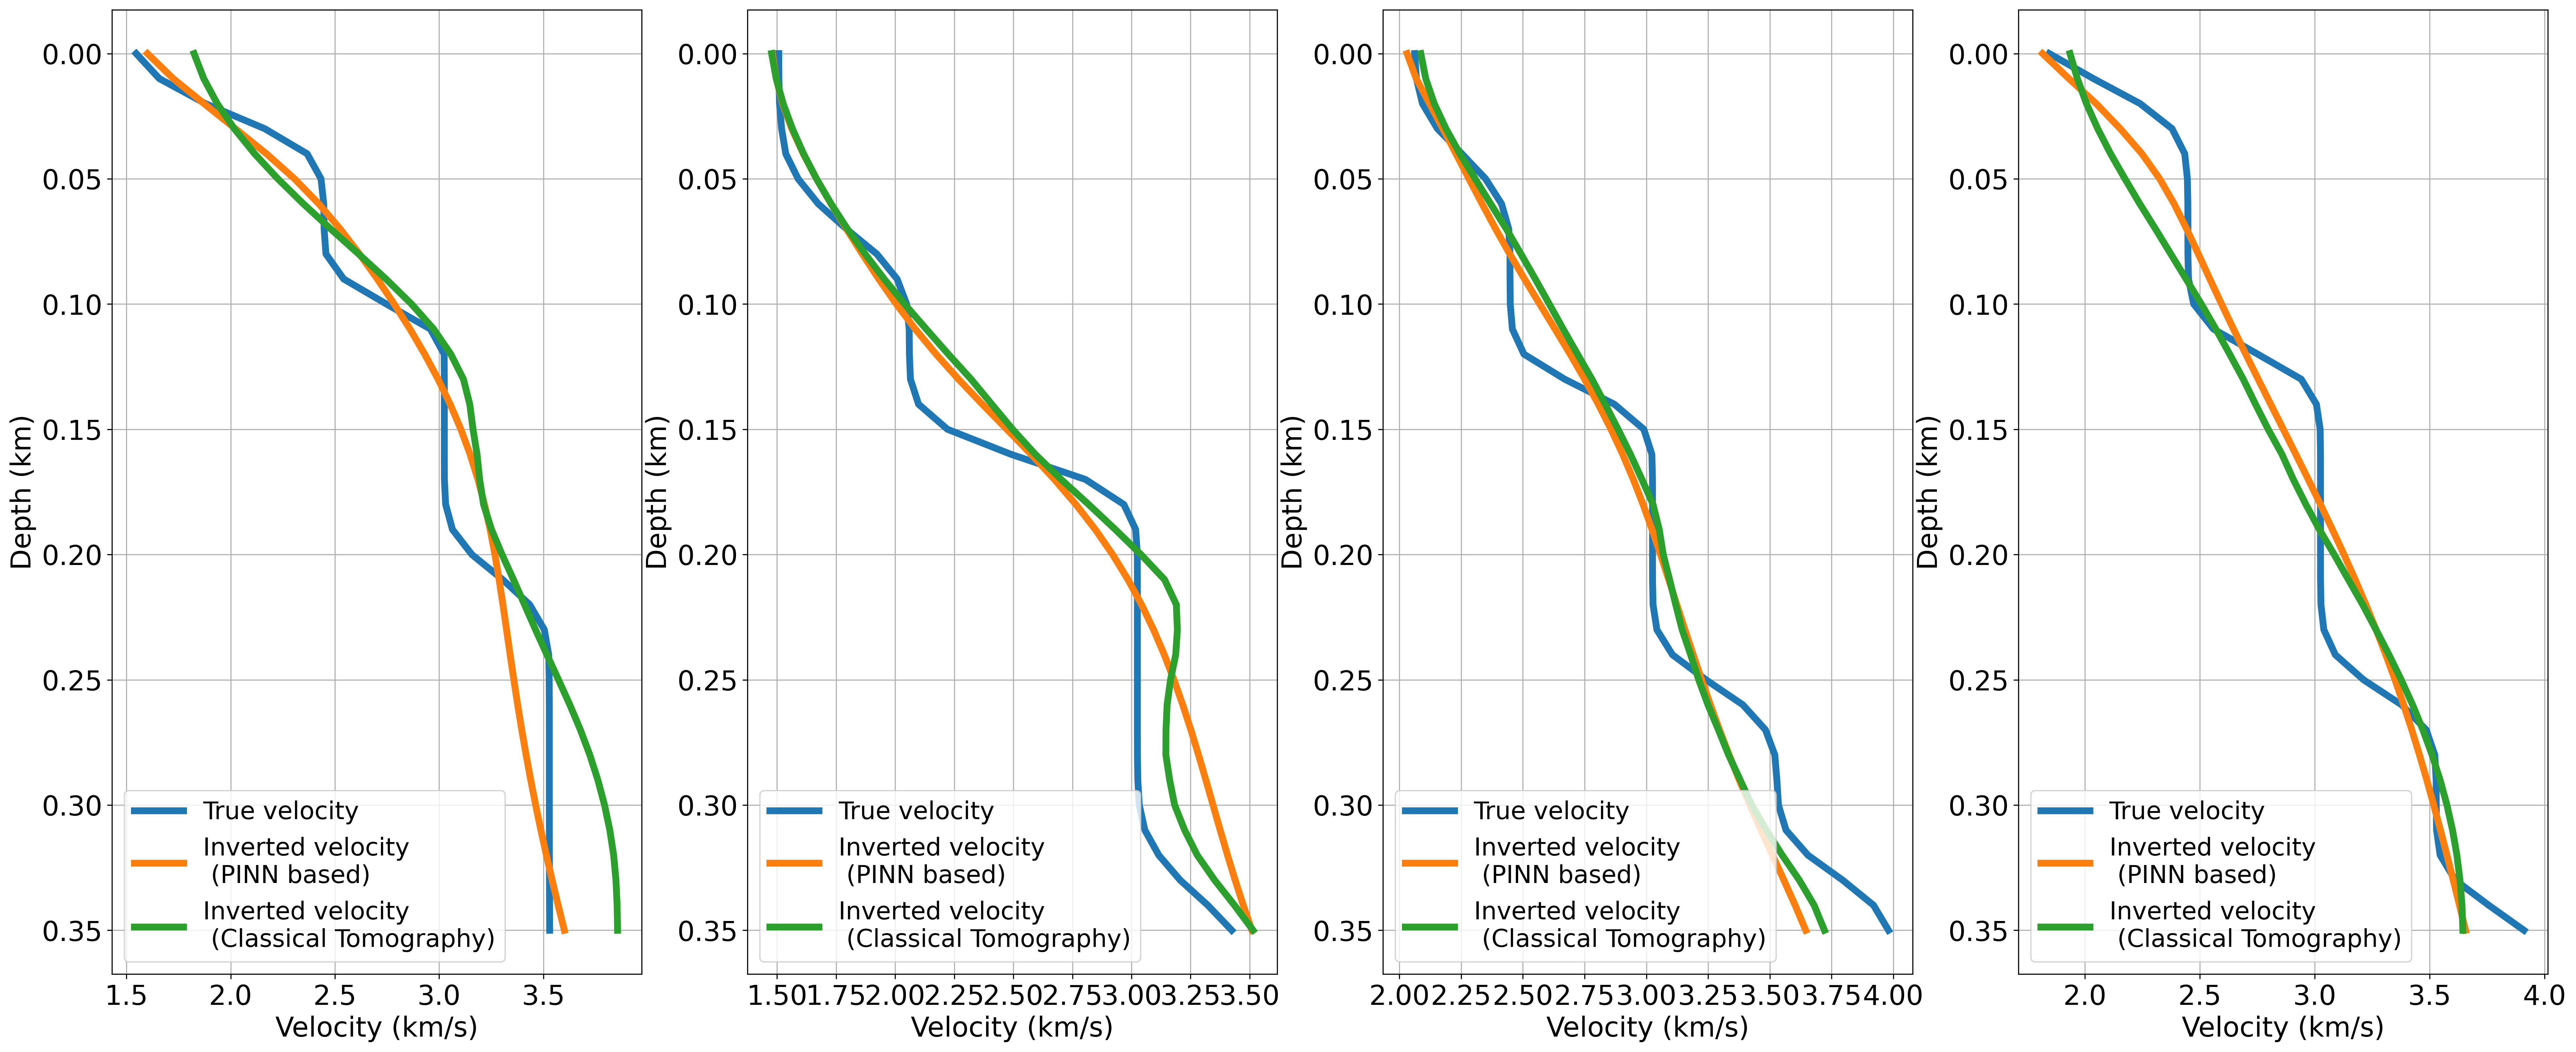
\includegraphics[width=0.9\textwidth]{figures/chap03_pinn_enabled/example_2_profiles} 
 \caption{Vertical velocity profiles at 0.4 km, 0.9 km, 1.3 km and 1.9 km from left to right respectively for the second example.}
 \label{fig:example_2_profiles}
\end{figure}

\begin{figure}
       \centering
       \begin{subfigure}[b]{1.\textwidth}
               \centering
               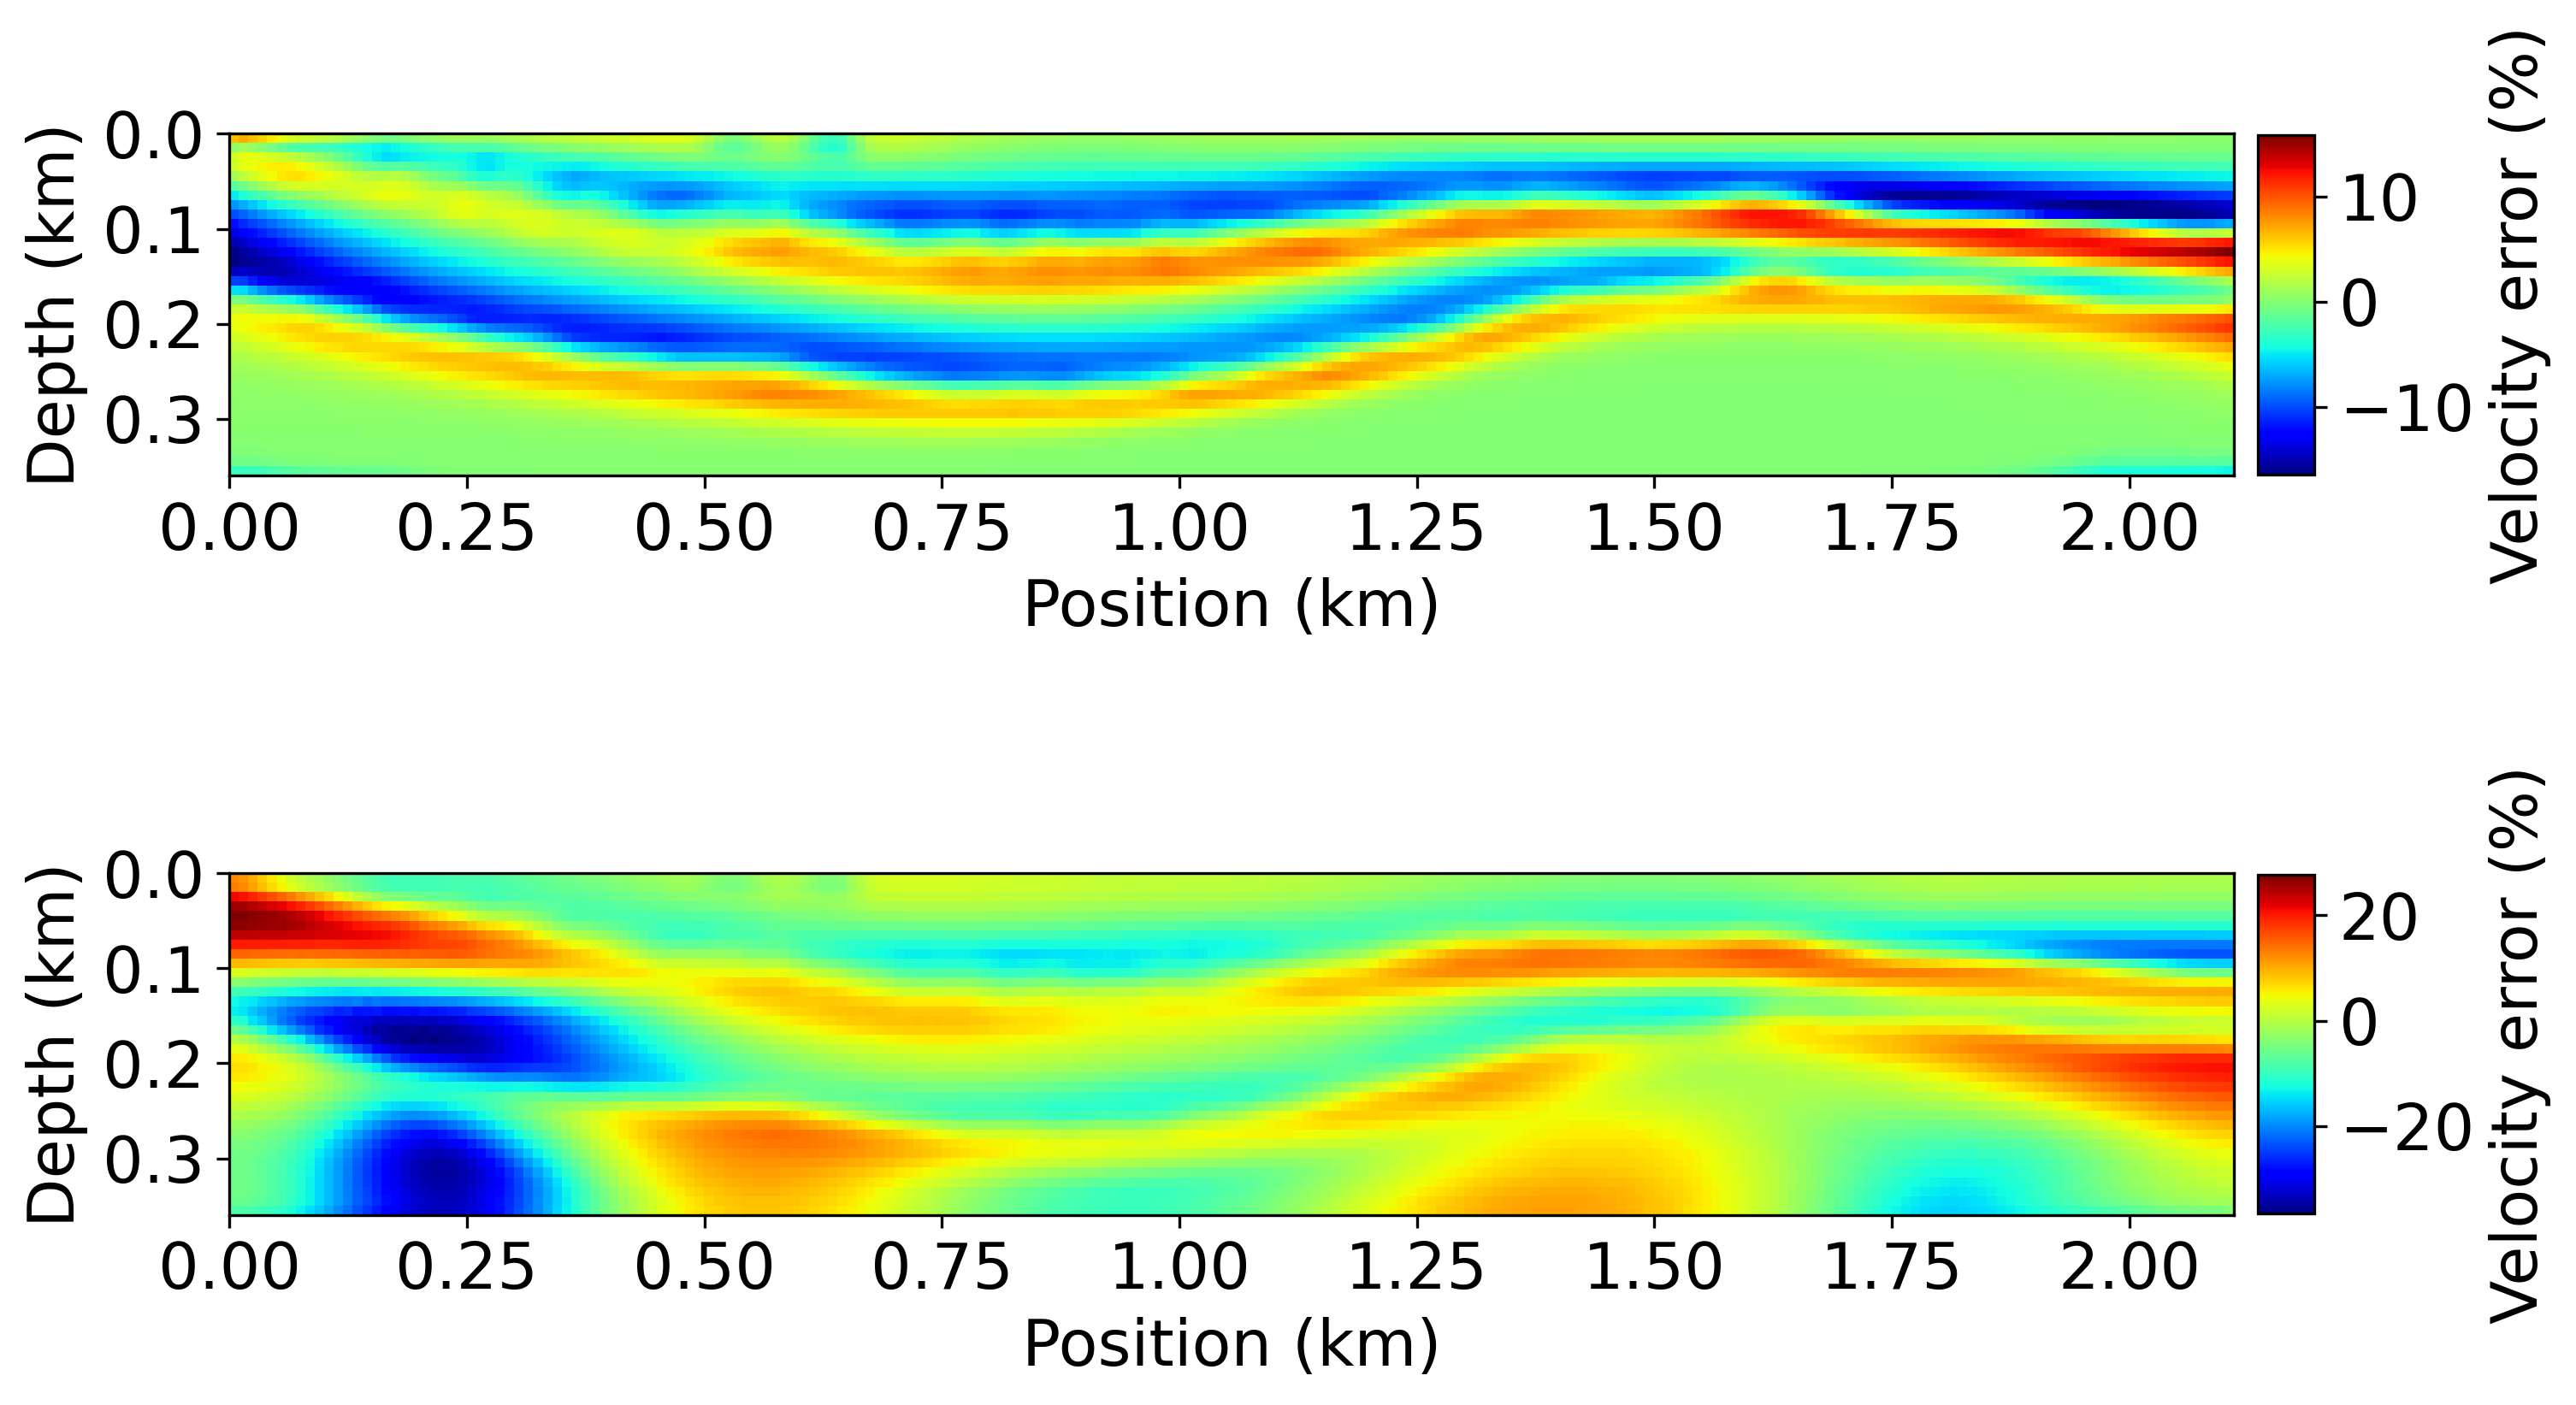
\includegraphics[width=\textwidth]{figures/chap03_pinn_enabled/example1_error} 
               \caption{}
               \label{fig:example1_error}
       \end{subfigure}
       %add desired spacing between images, e. g. ~, \quad, \qquad etc.
         %(or a blank line to force the subfigure onto a new line)
       \begin{subfigure}[b]{1.\textwidth}
               \centering
               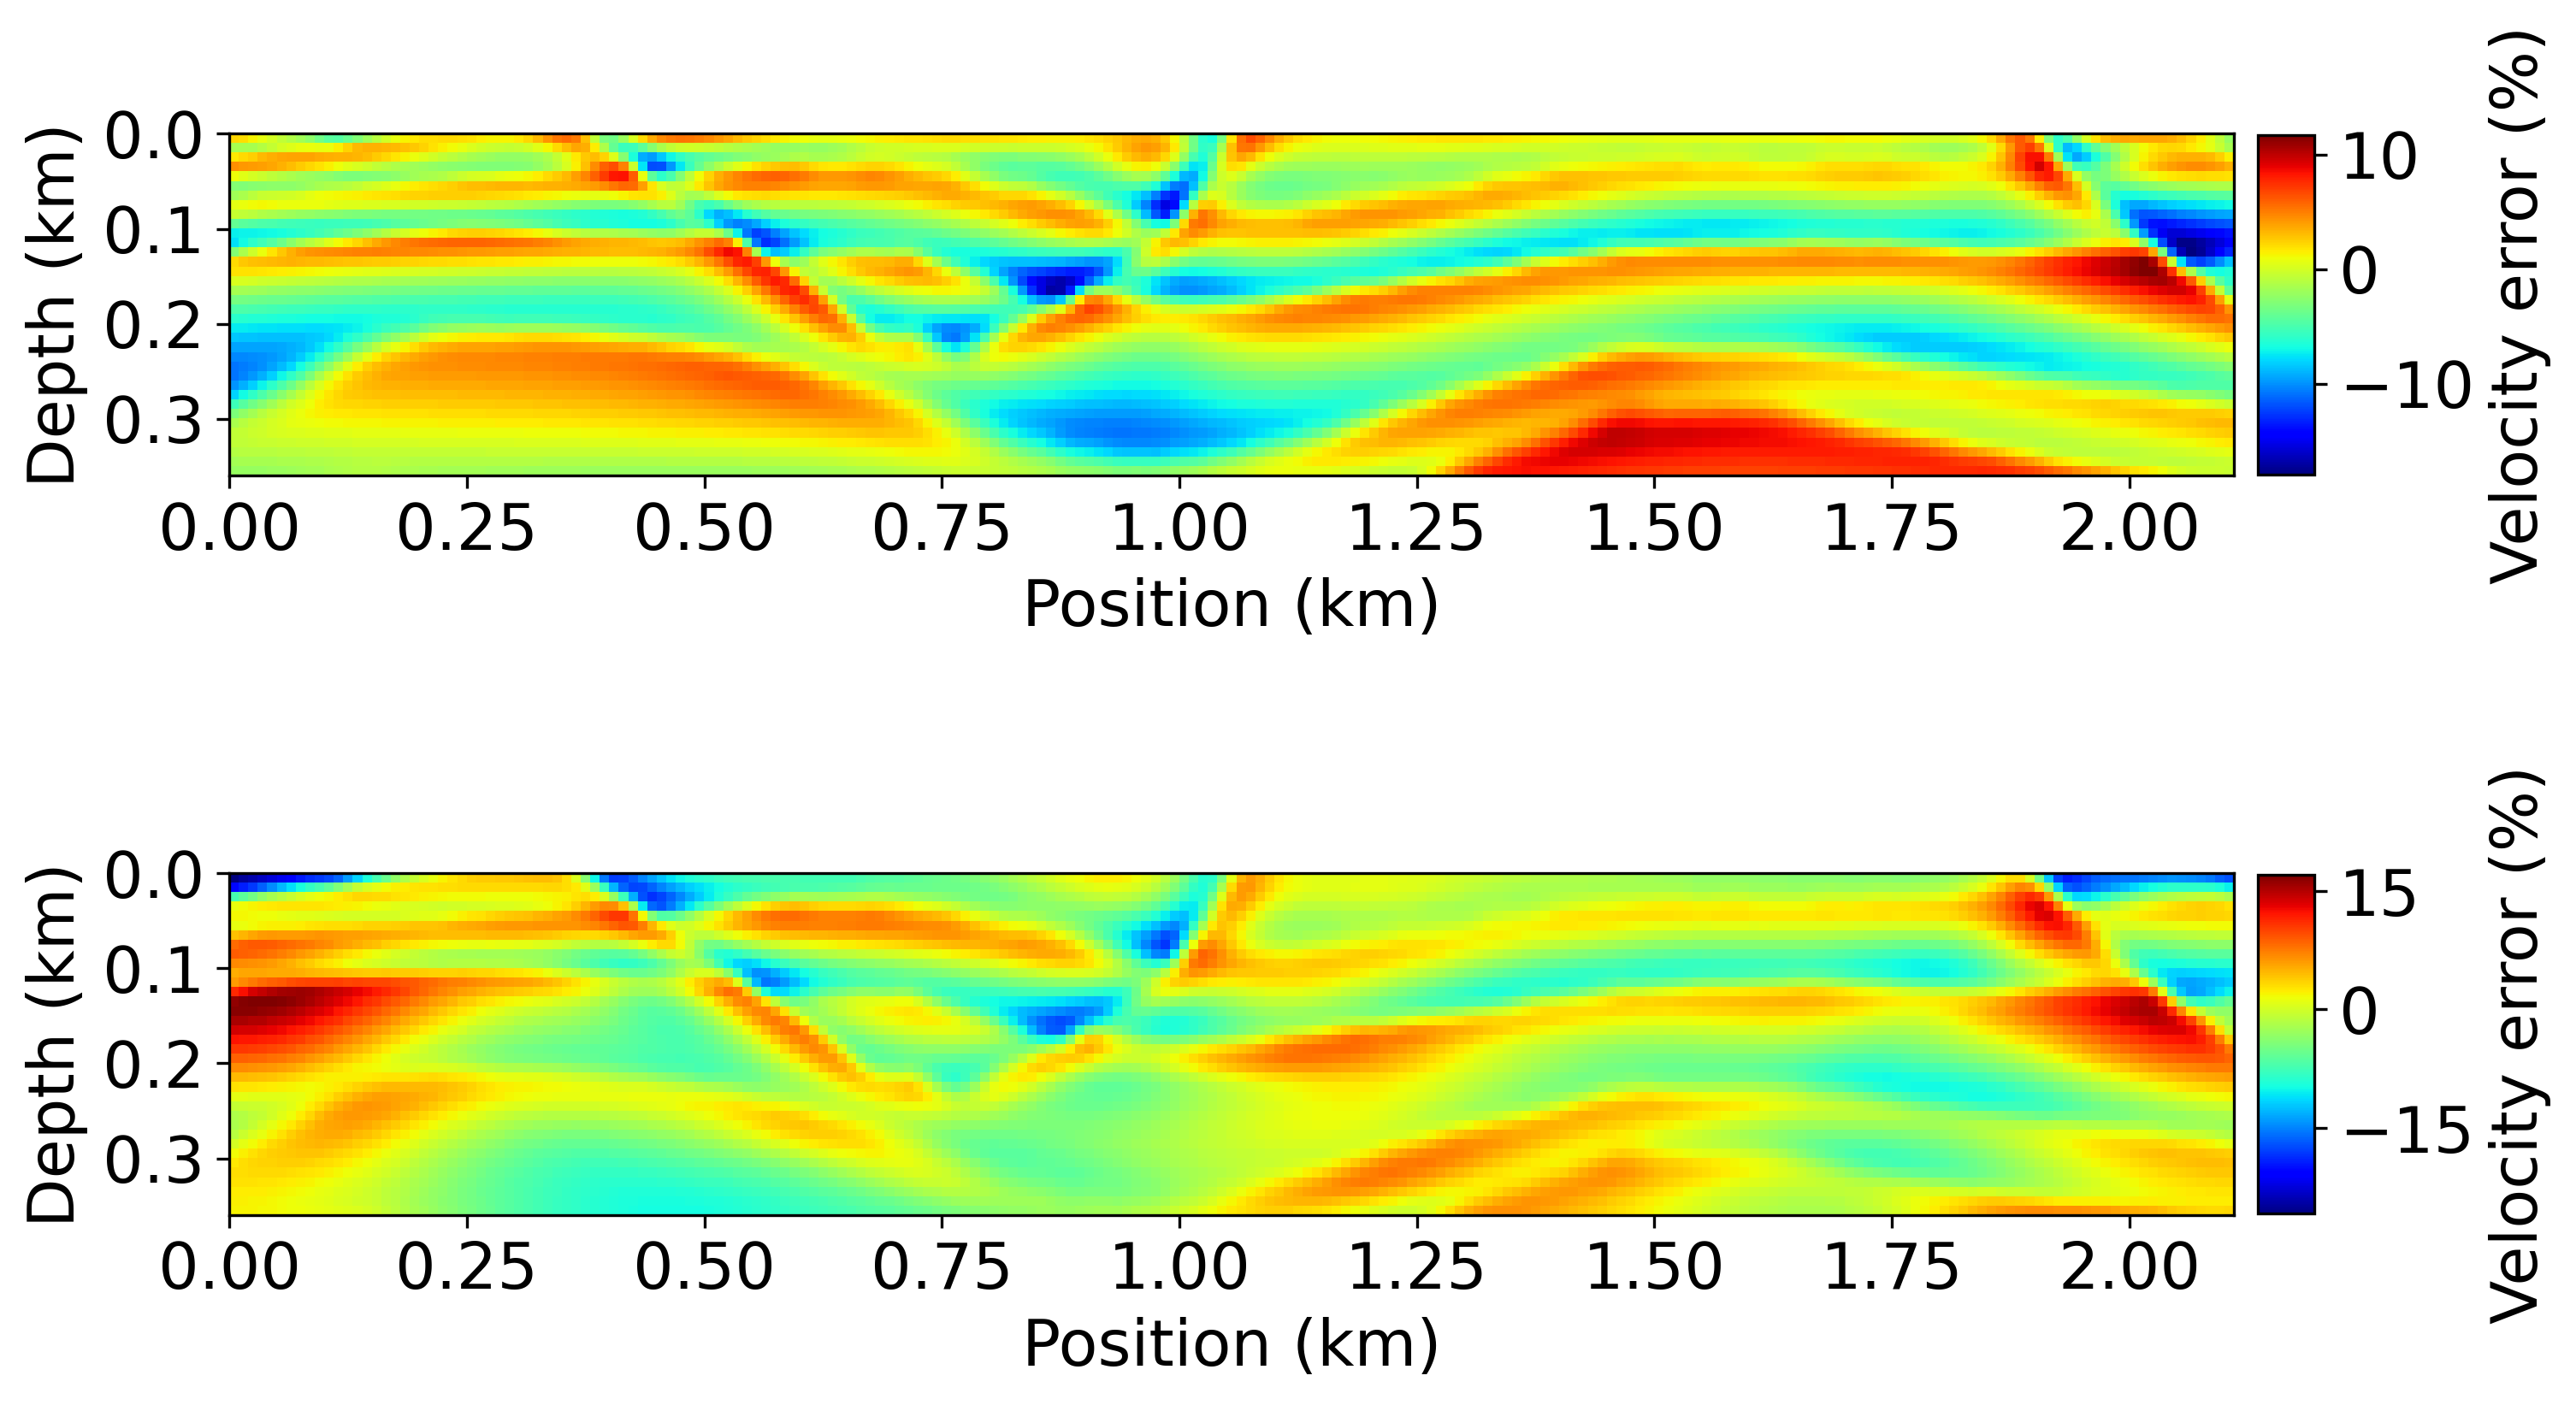
\includegraphics[width=\textwidth]{figures/chap03_pinn_enabled/example2_error}
               \caption{}
               \label{fig:example2_error}
       \end{subfigure}
       \caption{(a) Percentage error maps between the true model and the inversion results from the PINN approach (top) and the conventional approach (bottom) for the first example, and (b) for the second example, error map of PINN approach (top) and error map of conventional approach (bottom).}
       \label{fig:error}
\end{figure}
\section{Discussion}
\label{sec:discussion}

PINN-based traveltime tomography has clearly shown from the synthetic experiments that it can be used as a reliable tool alternative to conventional tomography. It has a significant advantage over the traditional tool in that it does not need to have a good initial guess which requires knowing a priori information on the investigated area. Nevertheless, the selection of hyperparameters (network architectures,  number of optimization iterations, minibatch size, weights of the loss components) plays an important role in the accuracy of the retrieved model. Among them, special attention needs to be paid to balance the weights of the loss components. I achieved robust convergence in the examples I showed by taking the weight of the data fitting term 100 times more than the PDE loss (eikonal) term. The influence of the weight of the regularizer on the problem is another important factor so that careful consideration needs to be given to decide the acceptable value for the weight of this specific term.  Therefore, optimizing the weights for each component of the loss along with the network weights could be a solution to this issue thus removing the need for time-consuming trial-and-error tasks.
\chapter{INTRODUCTION}
\label{chap:intro}



\input{chap_04/area_and_data }
%\chapter{INTRODUCTION}
\label{chap:intro}





%
% References in Bibtex format goes into below indicated file with .bib extension
\bibliography{myBiblio} % filename: myBiblio.bib
% You can use full name of authors, 
% however most likely some of the Bibtex entries you will find, 
% will use abbreviated first names.
% If you don't want to correct each of them by hand, 
% you can use abbreviated style for all of the references
%\bibliographystyle{abbrv}
% However, IAM suggests to use
\bibliographystyle{iamBiblioStyle} % better than to use {plain or abbrv}

%%% APPENDIXES
\appendix
%
% input your appendix
% If you are not using minted style, then comment the first appendix below
% otherwise uncomment.
%uncomment%  \chapter{Proof of Some Theorem}
\label{app:mintedCodes}

This is appendix text.

\definecolor{myBgColour}{rgb}{0.99,0.99,0.99} % almost white

\setminted[python]{frame=single,
framesep=2mm,
baselinestretch=1.1,
bgcolor=myBgColour,
fontsize=\footnotesize,
linenos, autogobble,
python3=true}

\setminted[matlab]{frame=single,
framesep=2mm,
baselinestretch=1.1,
bgcolor=myBgColour,
fontsize=\footnotesize,
linenos, autogobble,
python3=true}

%\captionsetup[Listing]{format=plain,font={small},labelfont={bf}, aboveskip=-5px}
%\renewcommand{\theListing}{{\arabic{Listing}}}
%\setcounter{Listing}{0}


However, we place a python code here with a listing environment
Listing~\ref{lst:first}.	

\begin{listing}	
\begin{minted}{python}
# Python program to check if the input number is prime or not

num = 407

# take input from the user
# num = int(input("Enter a number: "))

# prime numbers are greater than 1
if num > 1:
   # check for factors
   for i in range(2,num):
       if (num % i) == 0:
           print(num,"is not a prime number")
           print(i,"times",num//i,"is",num)
           break
   else:
       print(num,"is a prime number")
       
# if input number is less than
# or equal to 1, it is not prime
else:
   print(num,"is not a prime number")
\end{minted}
\caption{This is the caption of this Listing environment\label{lst:first}}
\end{listing}

Also we wish to insert a MATLAB code, too.

\definecolor{myBackgroundColour}{rgb}{0.9,0.9,0.9} % almost gray
\begin{minted}[
frame=lines,
framesep=2mm,
baselinestretch=1.2,
bgcolor=myBackgroundColour,
fontsize=\footnotesize,
linenos
]{matlab}
function result = myprime(n)
% MATLAB program to check if the input number is prime or not

%% initially set output flag to true
 result = true;
%% iterate over all positive integers 2,3,...,n-1
%% if n is not divisible by any of these factors....it is prime
 if (n == 1)
     result = 'false';
 elseif (n == 2)
     result = 'true';
 else 
    for i=2:n-1,
        if (mod(n,i)==0)
           result = 'false';
        end
    end
 end
%% return "true" or "false" instead of 1 or 0  
 if (result)
    result = 'true';
 else
    result = 'false';
 end
\end{minted}


Furthermore, here are two files (myPythonCode.py and myMatlabCode.m) included.

\inputminted[
frame=single,
framesep=2mm,
baselinestretch=1.2,
bgcolor=myBackgroundColour,
fontsize=\footnotesize,
linenos
]{python}{myPythonCode.py}

\definecolor{myRed}{rgb}{0.95,0.1,0.1}

\begin{listing}
\inputminted[frame=single, linenos, bgcolor=myRed]{matlab}{myMatlabCode.m}
\caption{Here is the caption again}
\end{listing} % includes minted package examples!
%\chapter{Proof of Some Theorem}
\label{app:somethms}

This is appendix text.

\begin{listing}
  %\VerbListingBoxed{myMatlabCode.m}
  \VerbatimInput{myMatlabCode.m}
	%\inputminted{matlab}{myMatlabCode.m} % only if minted is used!
  %\VerbListing{myMatlabCode.m}
\caption{The \texttt{lintest} function in a floating ``listing'' environment.}
\label{mfile:linetest-3}
\end{listing}


%
%
% If you are a Ph.D. Student you need to insert a CV at the end of you thesis
% Check vita.tex for a simple CV template in Latex
%\curriculumvitae
\label{chapter:vita}

\section*{\uppercase{Personal Information}}

\textbf{Surname, Name: } Surname, Name\\
\textbf{Nationality:} Turkish (TC) \\
\textbf{Date and Place of Birth:} dd.mm.yyyy, City\\
\textbf{Marital Status:} Single \\
\textbf{Phone:} 0 312 0000000 \\
\textbf{Fax:} 0 312 0000000 \\

\section*{\uppercase{Education}}

\begin{tabular}{lll}
\textbf{Degree} & \textbf{Institution} & \textbf{Year of Graduation} \\
M.S. & M.S. Institute & M.S. Year \\
B.S. & B.S. Institute & B.S. Year \\
High School & High School Name & High School Graduating Year
\end{tabular}

\section*{\uppercase{Professional Experience}}

\begin{tabular}{lll}
\textbf{Year} & \textbf{Place} & \textbf{Enrollment} \\
Duration 1 & Institute/Company 1 & Role/Position/Experience 1 \\
Duration 2 & Institute/Company 2 & Role/Position/Experience 2 
\end{tabular}

\section*{\uppercase{Publications}}
\subsection*{International Conference Publications}
Your publications goes here. Do not try to use Bibtex, since Bibtex builds a single bibliography
database for the document.

\end{document}
